\chapter{Технологический раздел}

%В данном разделе описан выбор системы управления базой данных, средств разработки серверной и клиентской частей ПО, интерфейсов и представлена общая схема взаимодействия компонентов системы. Также, описаны методы тестирования и обеспечения безопасности данных.

\section{Выбор СУБД}
\paragraph{Основные данные}\mbox{}

В качестве СУБД была выбрана бесплатная система управления базами данных PostgreSQL, поддерживаемая большинством операционных систем. PostgreSQL является реляционной~\cite{bib21} и поддерживает множество различных типов и структур данных, в том числе данные в текстовом формате JSON. Также с её помощью можно создавать пользовательские типы данных. PostgreSQL отвечает требованиям ACID, а также поддерживает различные виды ограничений, за счёт которых обеспечивается целостность данных системы, оконные функции, табличные функции и триггеры. БД Postgres является строковой, что означает высокую скорость выполнения запросов, обращающихся к отдельным записям. Листинги скриптов для работы с Postgres приведены в Приложении А.

\paragraph{Аналитические данные}\mbox{}

Для аналитических данных была выбрана колоночная СУБД ClickHouse. Она обеспечивает сжатие данных, автоматическое распараллеливание больших запросов по ресурсам предоставленного сервера и физическую сортировку данных по первичному ключу~\cite{bib22}. ClickHouse поддерживает декларативный язык запросов на основе SQL, включая группировку, оконные функции, подзапросы и объединения. Данный вид БД обеспечивает высокую скорость запросов на агрегацию, что особенно важно для аналитических данных~\cite{bib18}. Листинги скриптов для работа с ClickHouse приведены в Приложении А.

Для таблиц был использован движок MergeTree как наиболее функциональный среди движков ClickHouse~\cite{bib30}. 

Для таблицы очереди событий был использован движок Kafka~\cite{bib29}, который работает с Apache Kafka. Это позволяет организовывать прямую связь топика в Kafka с таблицей ClickHouse, а следовательно: подписываться на потоки данных, организовать отказоустойчивое хранилище, обрабатывать события по мере их появления. При помощи данного движка реализуется массовая вставка данных~\cite{bib38}, что обеспечивает большую производительность и меньшую нагрузку при работе с колоночными СУБД.

\paragraph{Потоковые данные}\mbox{}

Для передачи данных о событиях в основной системе, которые можно отнести к потоковым данным, в хранилище ClickHouse был использован Apache Kafka~---~распределённый программный брокер сообщений с открытым исходным кодом для обработки потоковых данных в реальном времени с высокой пропускной способностью~\cite{bib23}. Также, Kafka был использован для подготовки рекламных сообщений к отправлению. В обоих случаях были созданы соответствующие топики, то есть виртуальные хранилища сообщений схожего содержания,~---~events для добавления событий в хранилище и ads для рассылки рекламы. Данные разных топиков обрабатываются параллельно, и внутри каждого топика Kafka автоматически партиционирует данные, что также обеспечивает параллельную обработку. В целом, в Kafka процессы генерирования, отправки и считывания сообщений организованы независимо друг от друга. Использование брокера обеспечивает видимое преимущество в скорости работы с потоками данных.

\section{Выбор средств разработки серверной и клиентской частей ПО}
Для разработки серверной части был выбран язык программирования Golang~\cite{bib24}. Выбор обусловлен наличием в Golang библиотек для тестирования ПО, работы с http протоколом~\cite{bib25}, взаимодействия с выбранными для хранения данных СУБД~\cite{bib26}, работы с JWT-токенами~\cite{bib28}, шифрования данных~\cite{bib27}, а также иных необходимых для реализации поставленных цели и задач средств.

В качестве SMTP сервера для рассылки почтовой рекламы был выбран Brevo~\cite{bib35}. По данным компании, 99,8\% всех отправленных с её платформы электронных писем, доставляются в течение 20 секунд. Также, одной из причин выбора стало то, что сервис предоставляет 300 бесплатных электронных писем в день при использовании бесплатного плана. Для рассылки был использован и подтверждён домен blurby.lownie.su.

Для разработки клиентской части был выбран фреймворк Vue.js~---~фреймворк для создания пользовательских интерфейсов, подходящий для реализации сложных одностраничных приложений~\cite{bib31}. Во Vue зависимости компонента автоматически отслеживаются при отрисовке, поэтому система отрисовывает только затронутые компоненты при изменении состояния в отличие от React~\cite{bib32}. По производительности Vue сравним с такими популярным фреймворками как React и Angular и является более производительным, чем AngularJS. Также, Vue проще многих других фреймворков по архитектуре. 

Был использован MVVM паттерн. Интерфейс перестраивается автоматически при изменении данных за счёт использования Vuex~\cite{bib36}: он служит централизованным хранилищем для всех компонентов приложения, изменяя представляемые пользователю данные предписанным образом.

\section{Выбор средств реализации API}
Для реализации API взаимодействия серверной и клиентской частей продукта был использован Swagger~---~набор инструментов, созданных на основе спецификации OpenAPI, нужных при разработке, создании, документировании и использовании API \cite{bib33}. 

В файле спецификации были описаны пути запросов и соответствующие им методы и форматы запросов и ответов на запрос. При помощи OpenAPI Generator был сгенерирован серверный интерфейс, на основе которого были позже реализованы обработчики запросов \cite{bib34}.

Интерфейс взаимодействия серверной и клиентской частей представлен в таблице~\ref{table:api}.

\begin{table}[H]
\begin{center}
\caption{\label{table:api} Интерфейс взаимодействия серверной и клиентской частей}
\begin{tabular}{|l|c|l|} 
\hline
Путь          & Метод  & \multicolumn{1}{c|}{Описание}                     \\ \hline
/login        & post   & Вход пользователя в систему                       \\ \hline
/register     & post   & Регистрация пользователя                          \\ \hline
/events       & post   & Добавление информации о событии                   \\ \hline
/filter       & post   & Фильтрация событий                                \\ \hline
/users        & get    & Получение информации о всех пользователях \\ \hline
/clients      & get    & Получение информации о всех клиентах      \\ \hline
/client       & get    & Получение информации о клиенте            \\ \hline
/client       & post   & Регистрация клиента системы                       \\ \hline
/client       & delete & Удаление клиента из системы                       \\ \hline
/stats        & get    & Получение статистики системы                      \\ \hline
/user/id      & get    & Получение информации о пользователе по ID         \\ \hline
/user         & delete & Удаление пользователя                             \\ \hline
/user         & get    & Получение информации о пользователе по логину     \\ \hline
/user         & put    & Выдача пользователю прав администратора           \\ \hline
/event\_types & post   & Добавление типа события                           \\ \hline
/event\_types & get    & Получение типов событий                           \\ \hline
/ads          & post   & Создание рекламной рассылки                       \\ \hline
/ads          & get    & Получение рекламных рассылок                      \\ \hline
/users/me     & get    & Получение информации о текущем пользователе       \\ \hline
\end{tabular}
\end{center}
\end{table}

\newpage

\section{Взаимодействие компонентов и безопасность}

Взаимодействие серверной части с хранилищем было реализовано при помощи паттерна "Репозиторий". Разделение серверной логики и компонента доступа к данным позволяет без изменения кода подменять реализацию хранилища, обеспечивая удовлетворение обработчиков репозиториев заданному в логике интерфейсу.

Обобщённая схема взаимодействия компонентов изображена на рисунке~\ref{img:components}.

\begin{table}[h!]
  \centering
  \begin{tabular}{p{1\linewidth}}
    \centering
    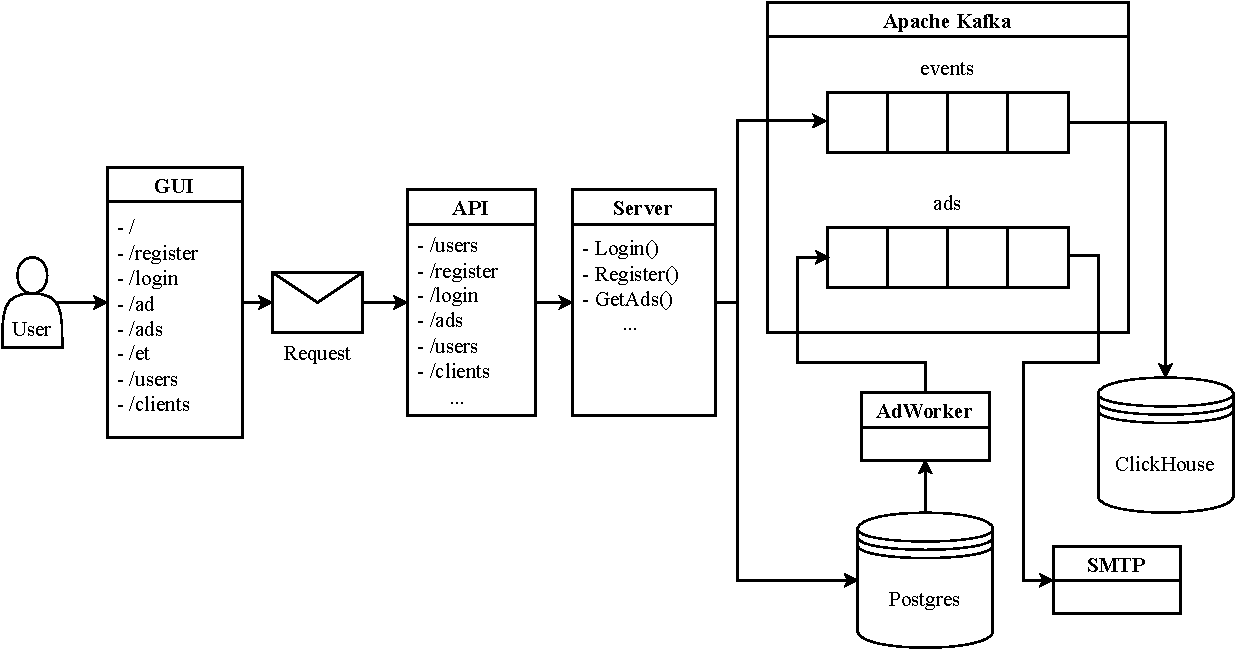
\includegraphics[width=1\linewidth]{./images/components.pdf}
    \captionof{figure}{Взаимодействие компонентов}
    \label{img:components}
  \end{tabular}
\end{table}

Для безопасности хранимых и передаваемых между компонентами данных были предусмотрены определённые средства защиты:
\begin{enumerate}
	\item Производится шифрование пароля с помощью хэш-функции bcrypt, пароль поступает в хранилище уже в зашифрованном виде.
	\item Ролевая модель ограничивает доступ пользователей к данным хранилища, если производится попытка их получения с подключения, не имеющего соответствующих прав.
	\item Производится аутентификация пользователя с помощью JWT-токена~---~ средства безопасной передачи информации посредством механизма подписи~---~назначаемого при успешном входе в систему~\cite{bib39}.
\end{enumerate}

\section{Web-интерфейс}

Web-интерфейс организован в формате одностраничного web-приложения или SPA. 

Таргетологу доступны:
\begin{enumerate}
	\item домашняя страница с просмотром статистики системы;
	\item страница формирования рекламной рассылки с настройками фильтрации;
	\item страница просмотра списка незавершённых рекламных рассылок;
	\item страница просмотра и создания типов событий, обрабатываемых системой.
\end{enumerate}

Администратору доступны:
\begin{enumerate}
	\item домашняя страница с просмотром статистики системы;
	\item страница просмотра и редактирования списка всех пользователей системы;
	\item страница просмотра и редактирования списка всех клиентов системы.
\end{enumerate}

%На рисунках~\ref{img:home}~--~\ref{img:clients} представлен реализованный web-интерфейс.

В приложении Б представлен реализованный web-интерфейс.

%\begin{figure}[h!]
%	\centering
%    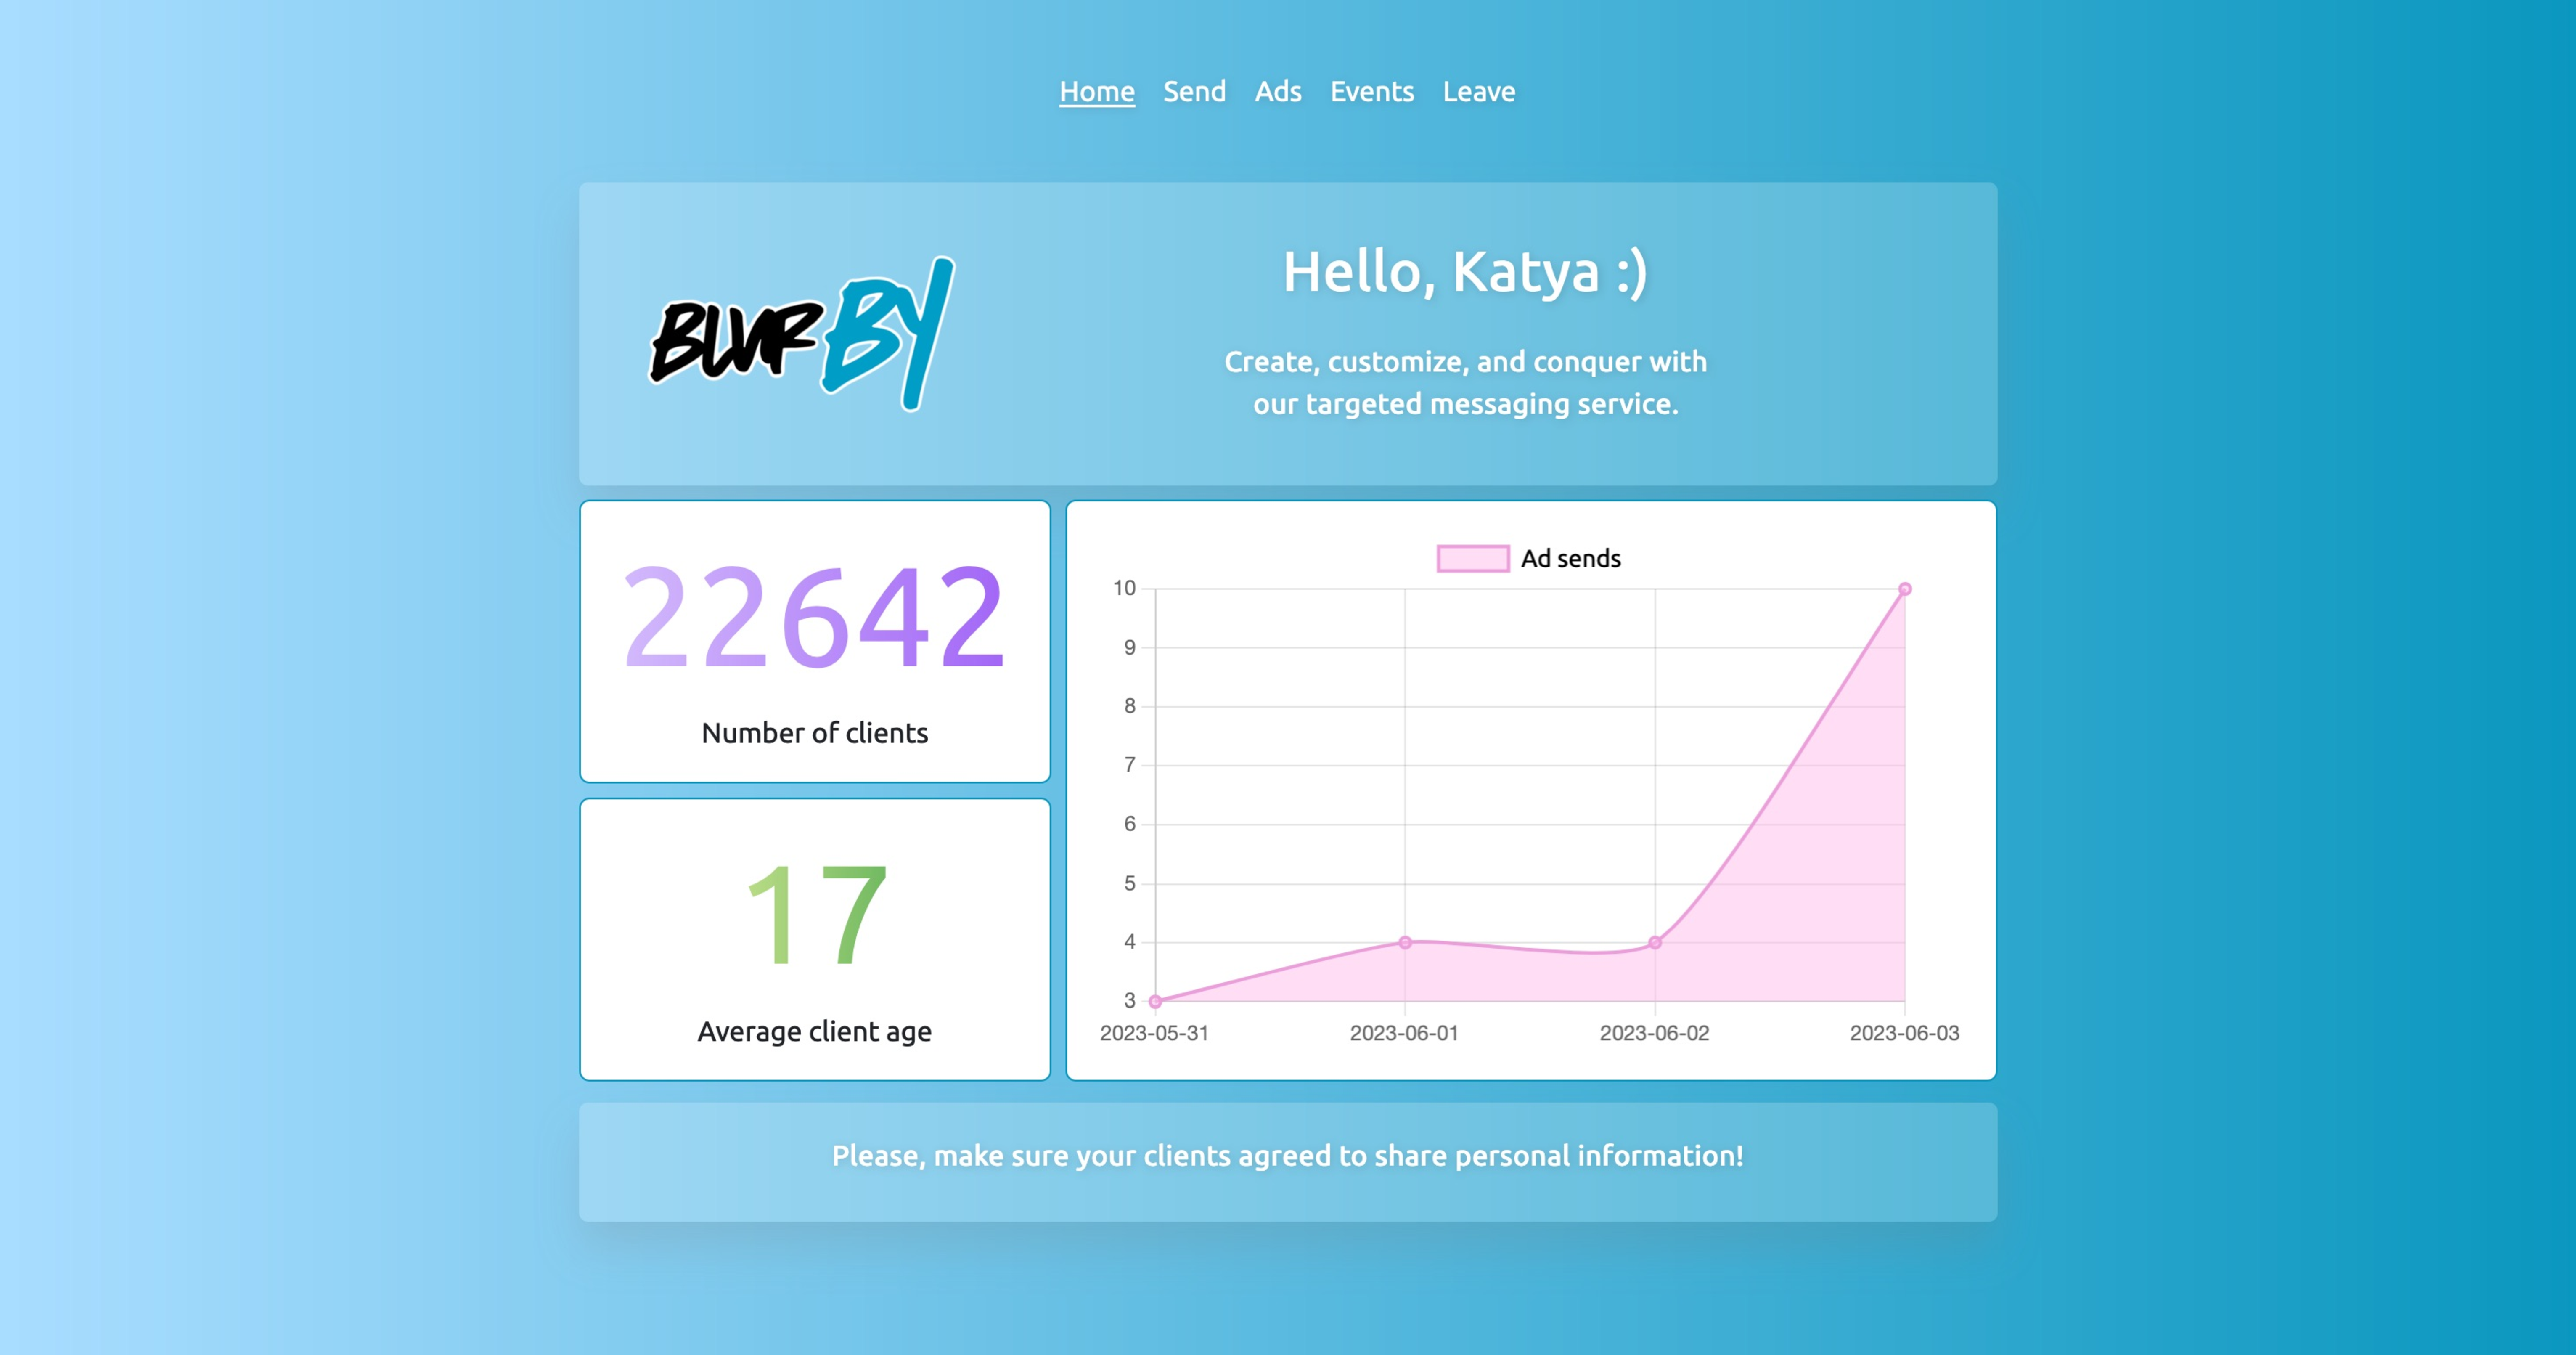
\includegraphics[width=0.8\linewidth]{./images/home.pdf}
%    \caption{Домашняя страница}
%    \label{img:home}
%\end{figure}
%
%%\begin{table}[h!]
%%  \centering
%%  \begin{tabular}{p{1\linewidth}}
%%    \centering
%%    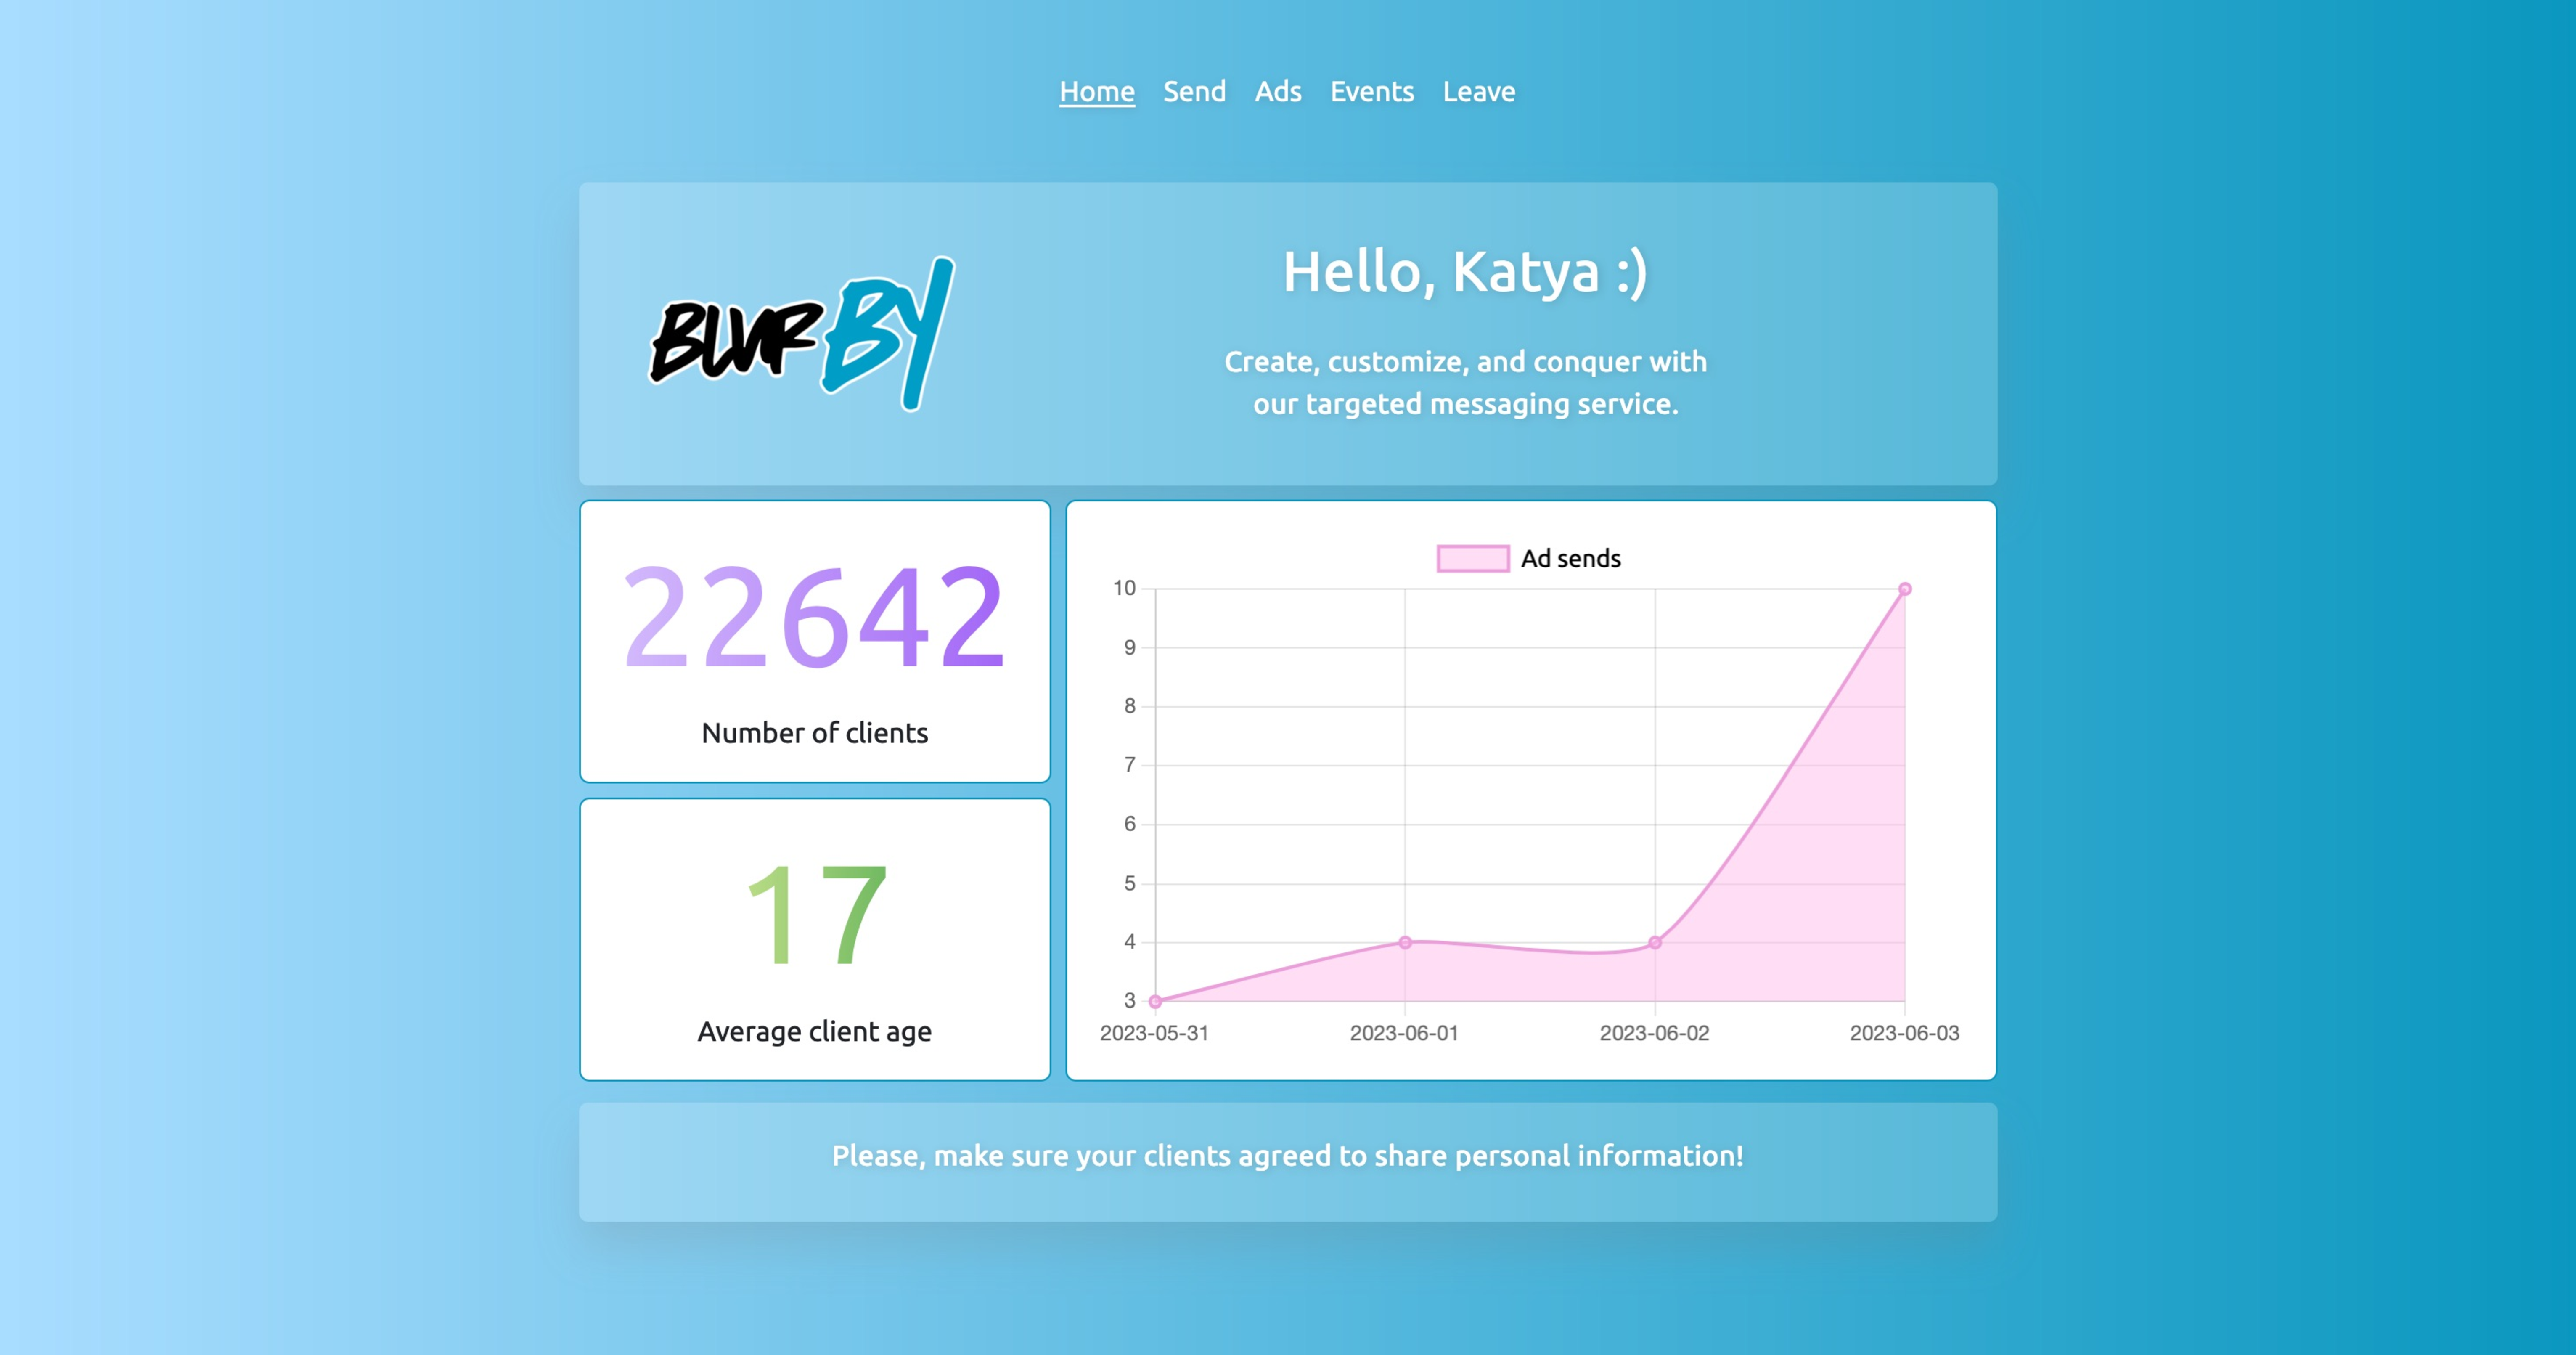
\includegraphics[width=0.8\linewidth]{./images/home.pdf}
%%    \captionof{figure}{Домашняя страница}
%%    \label{img:home}
%%  \end{tabular}
%%\end{table}
%
%\newpage
%%
%%\noindent
%
%\begin{figure}[h!]
%	\centering
%    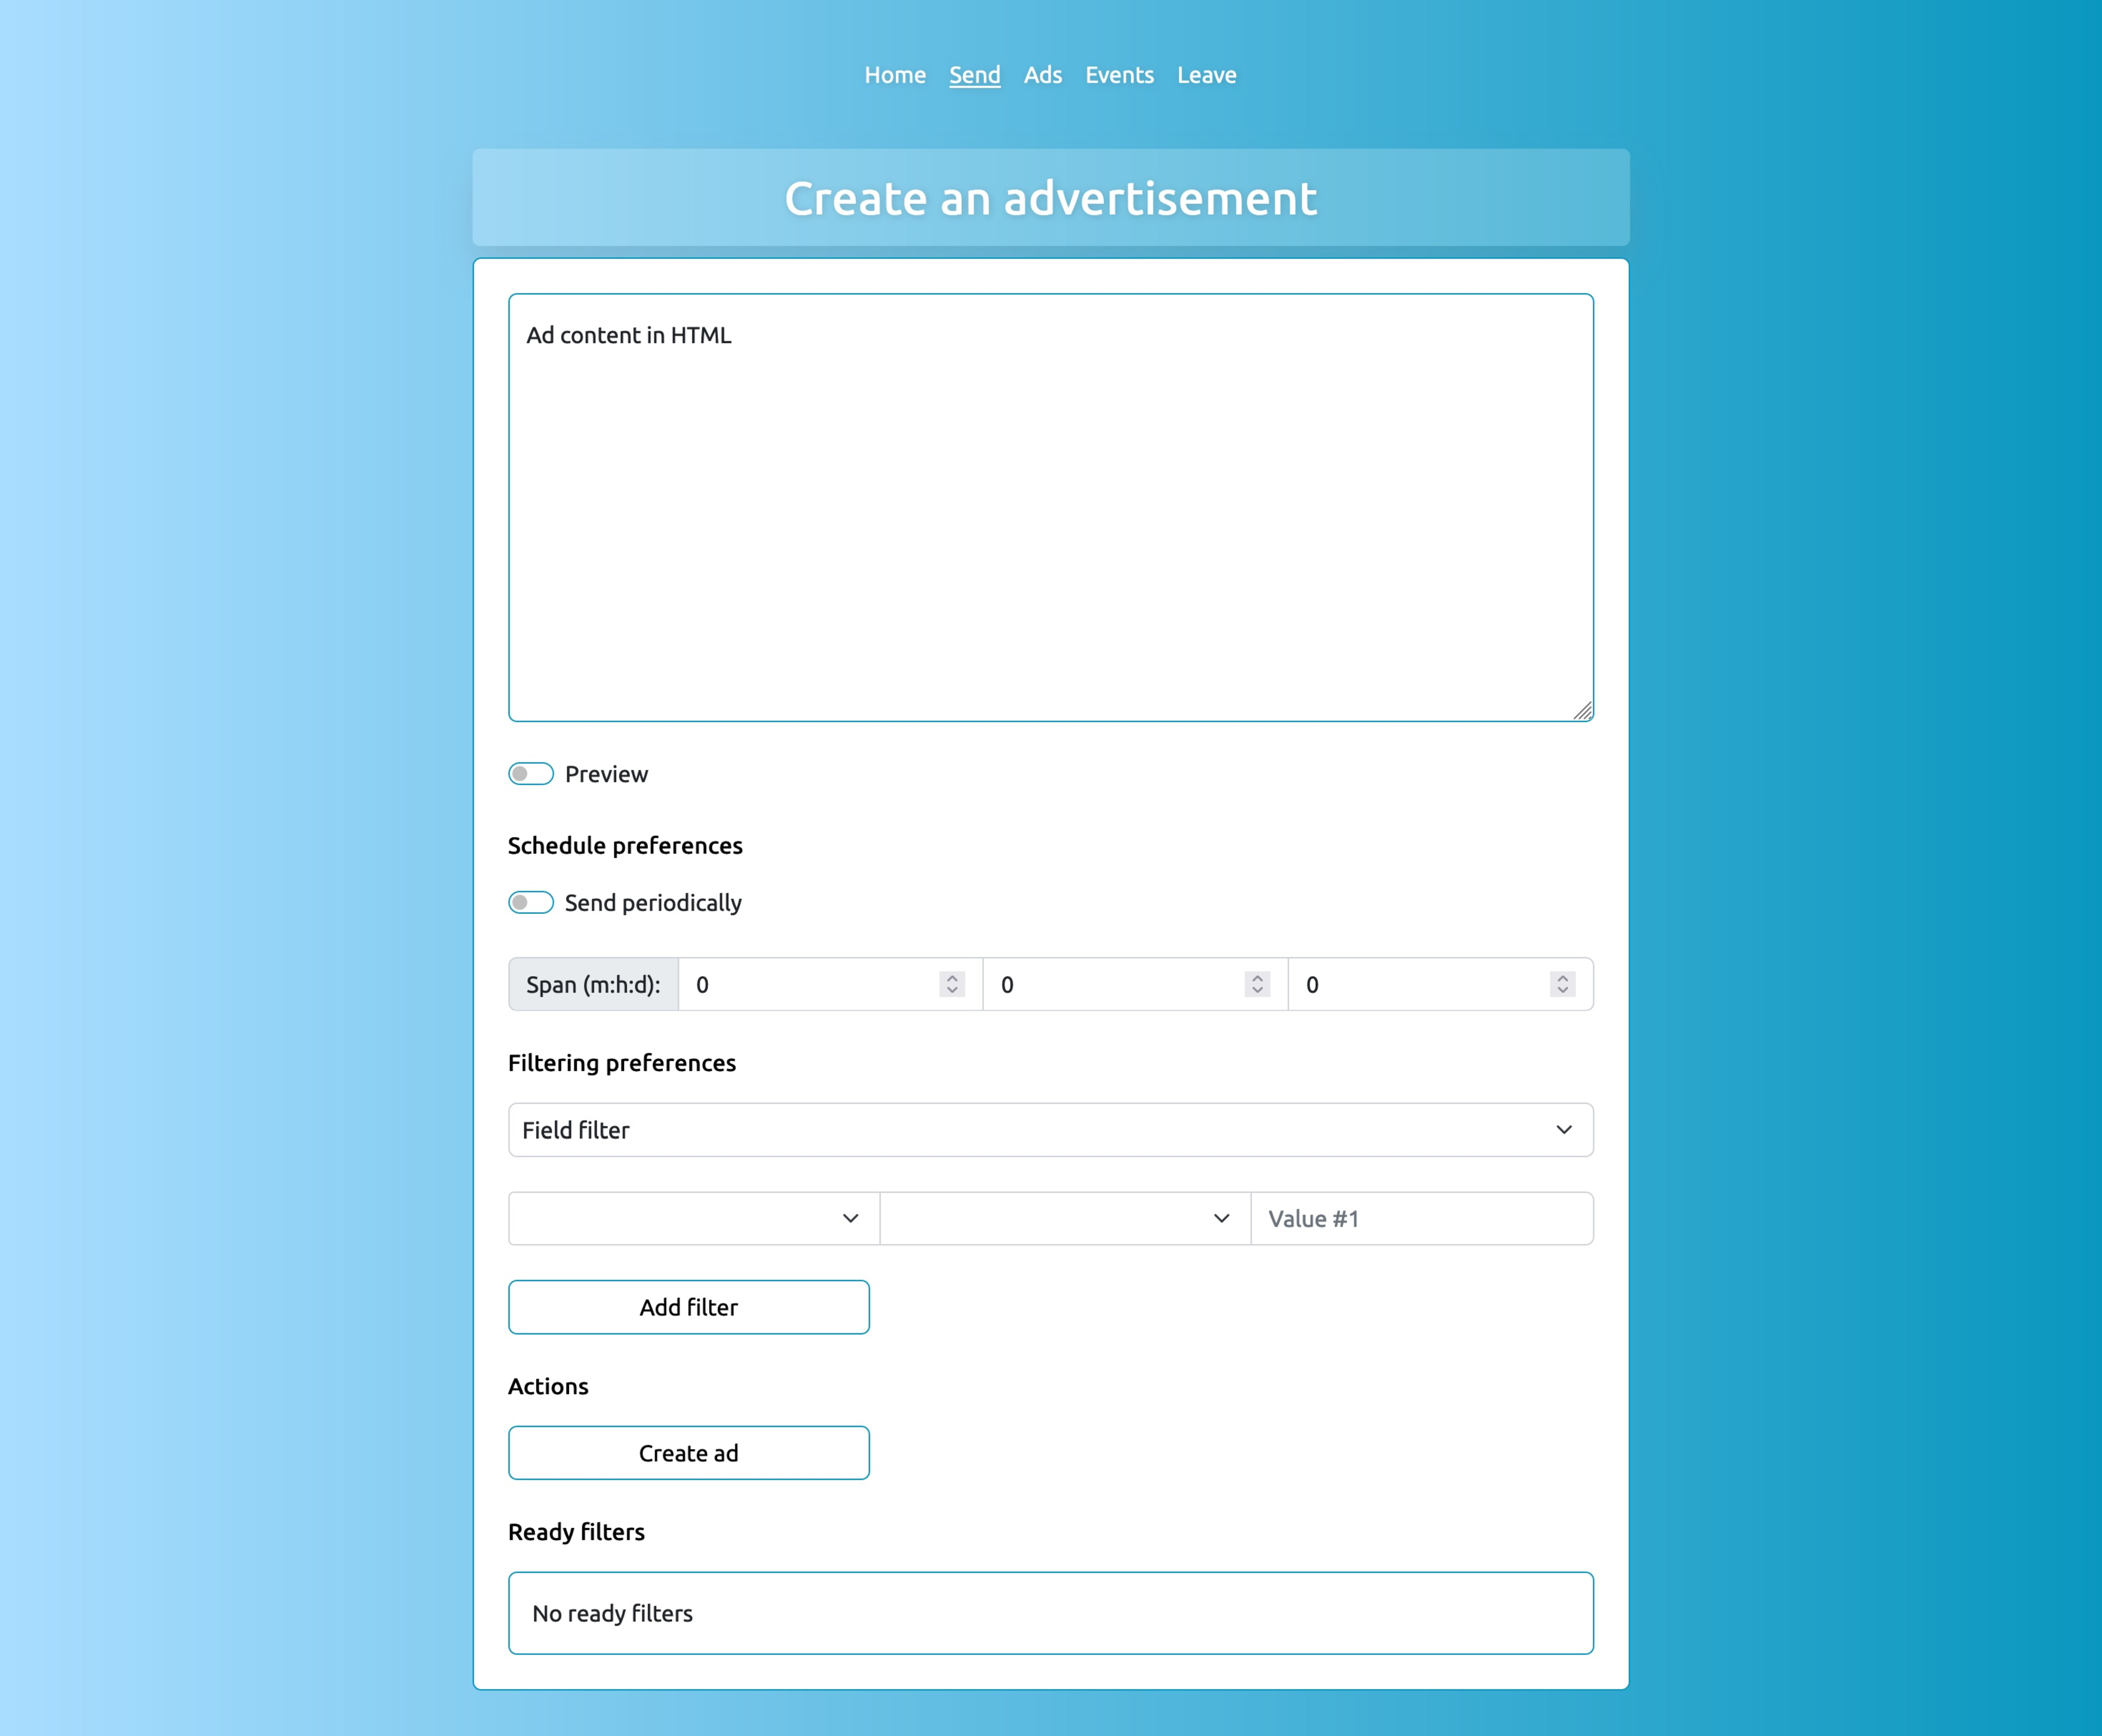
\includegraphics[width=\linewidth]{./images/ad.pdf}
%    \caption{Страница формирования рекламной рассылки}
%    \label{img:ad}
%\end{figure}
%
%%\begin{table}[h!]
%%  \centering
%%  \begin{tabular}{p{1\linewidth}}
%%    \centering
%%    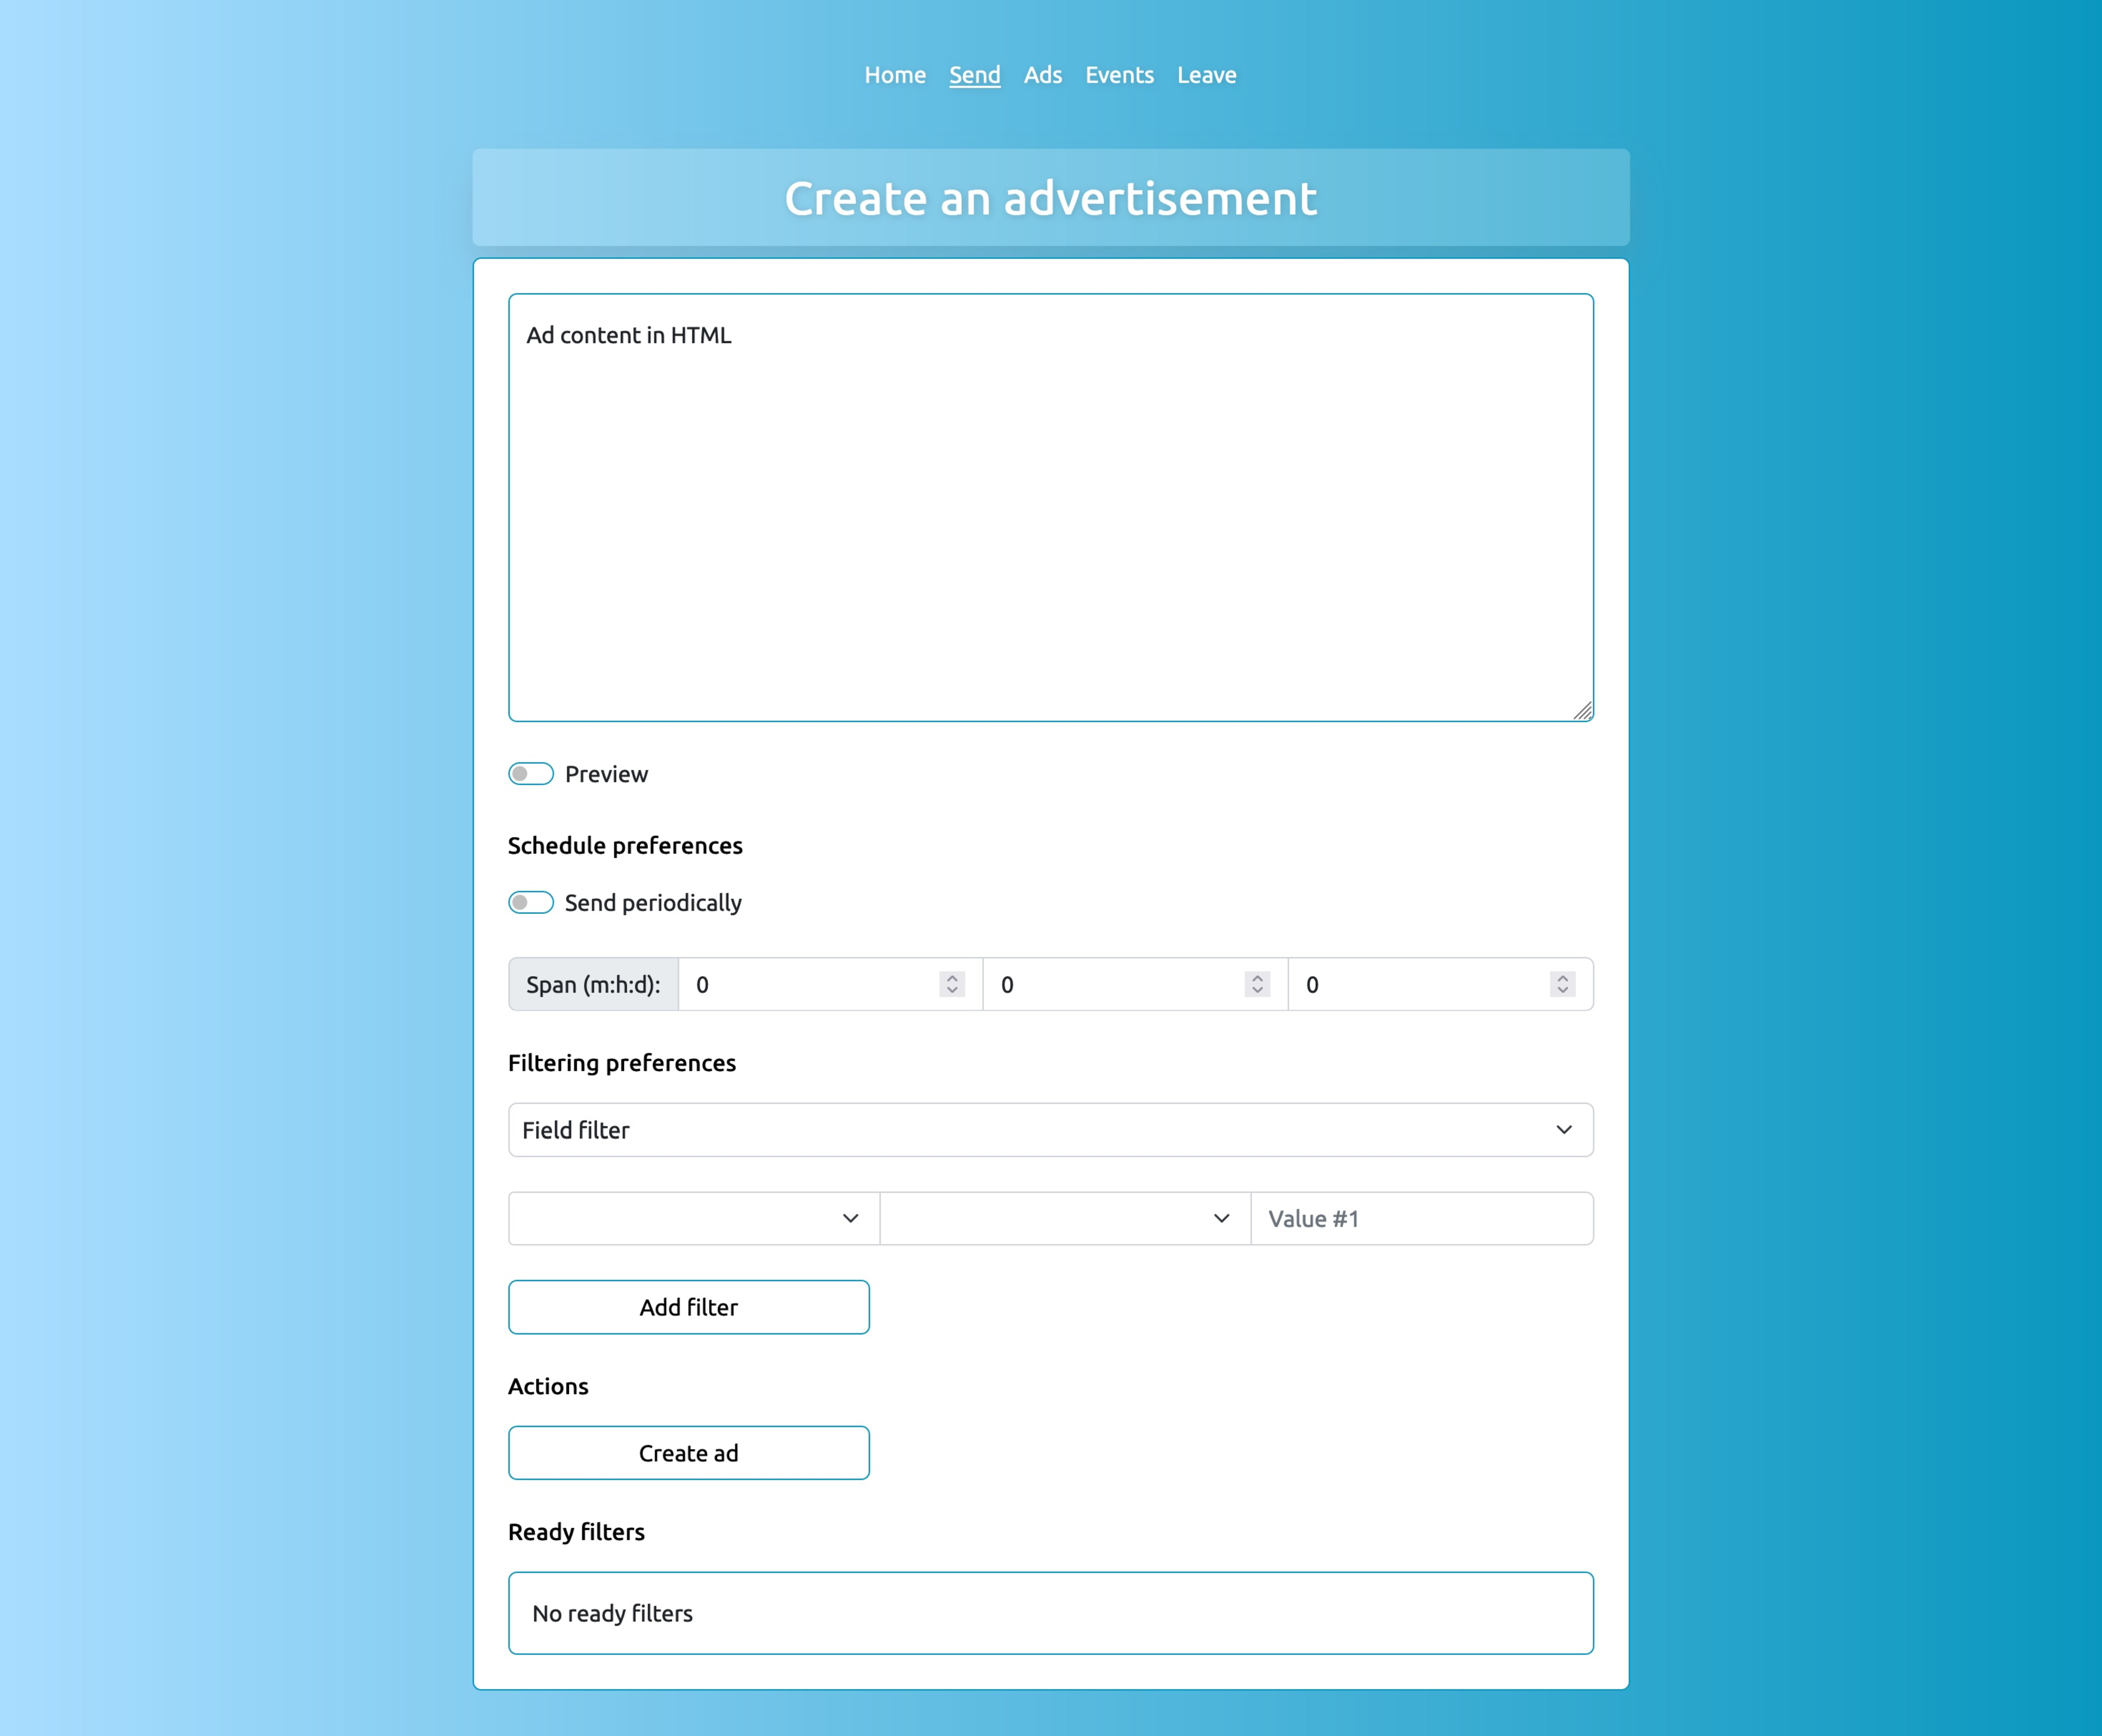
\includegraphics[width=0.8\linewidth]{./images/ad.pdf}
%%    \captionof{figure}{Страница формирования рекламной рассылки}
%%    \label{img:ad}
%%  \end{tabular}
%%\end{table}
%
%
%\begin{figure}[h!]
%	\centering
%    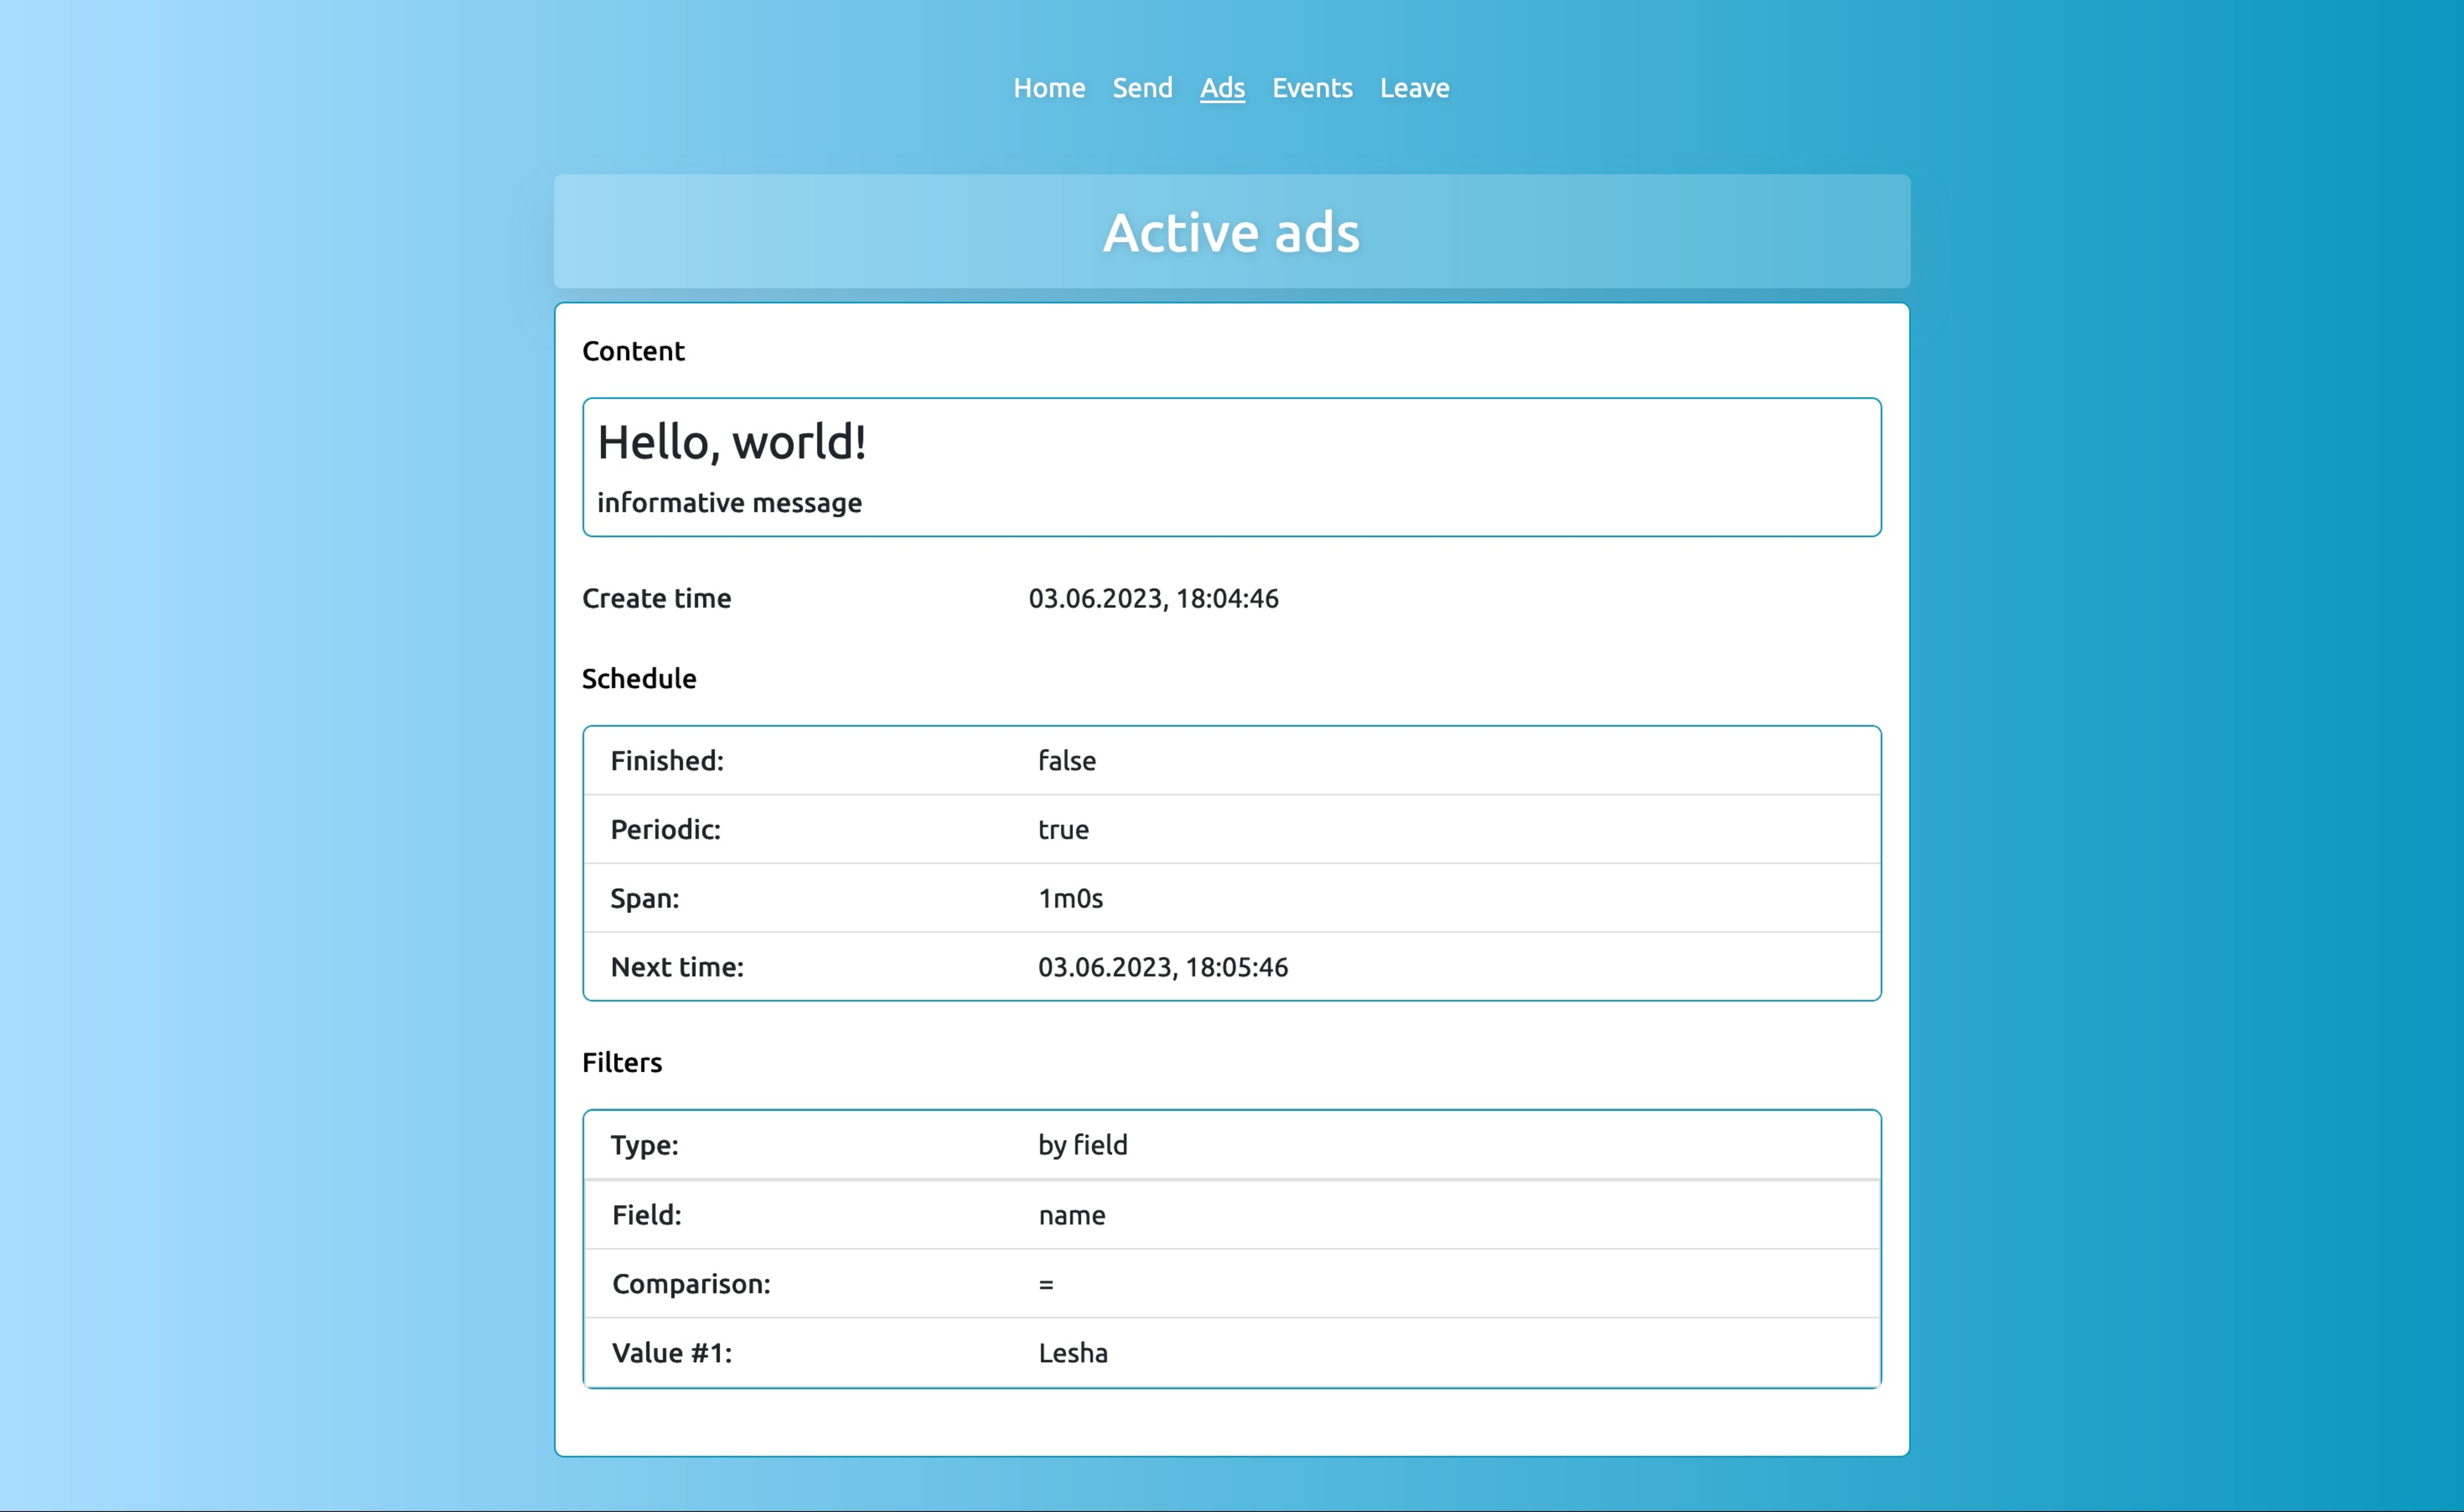
\includegraphics[width=\linewidth]{./images/ads.pdf}
%    \caption{Страница просмотра списка незавершённых рассылок}
%    \label{img:ads}
%\end{figure}
%
%%\begin{table}[h!]
%%  \centering
%%  \begin{tabular}{p{1\linewidth}}
%%    \centering
%%    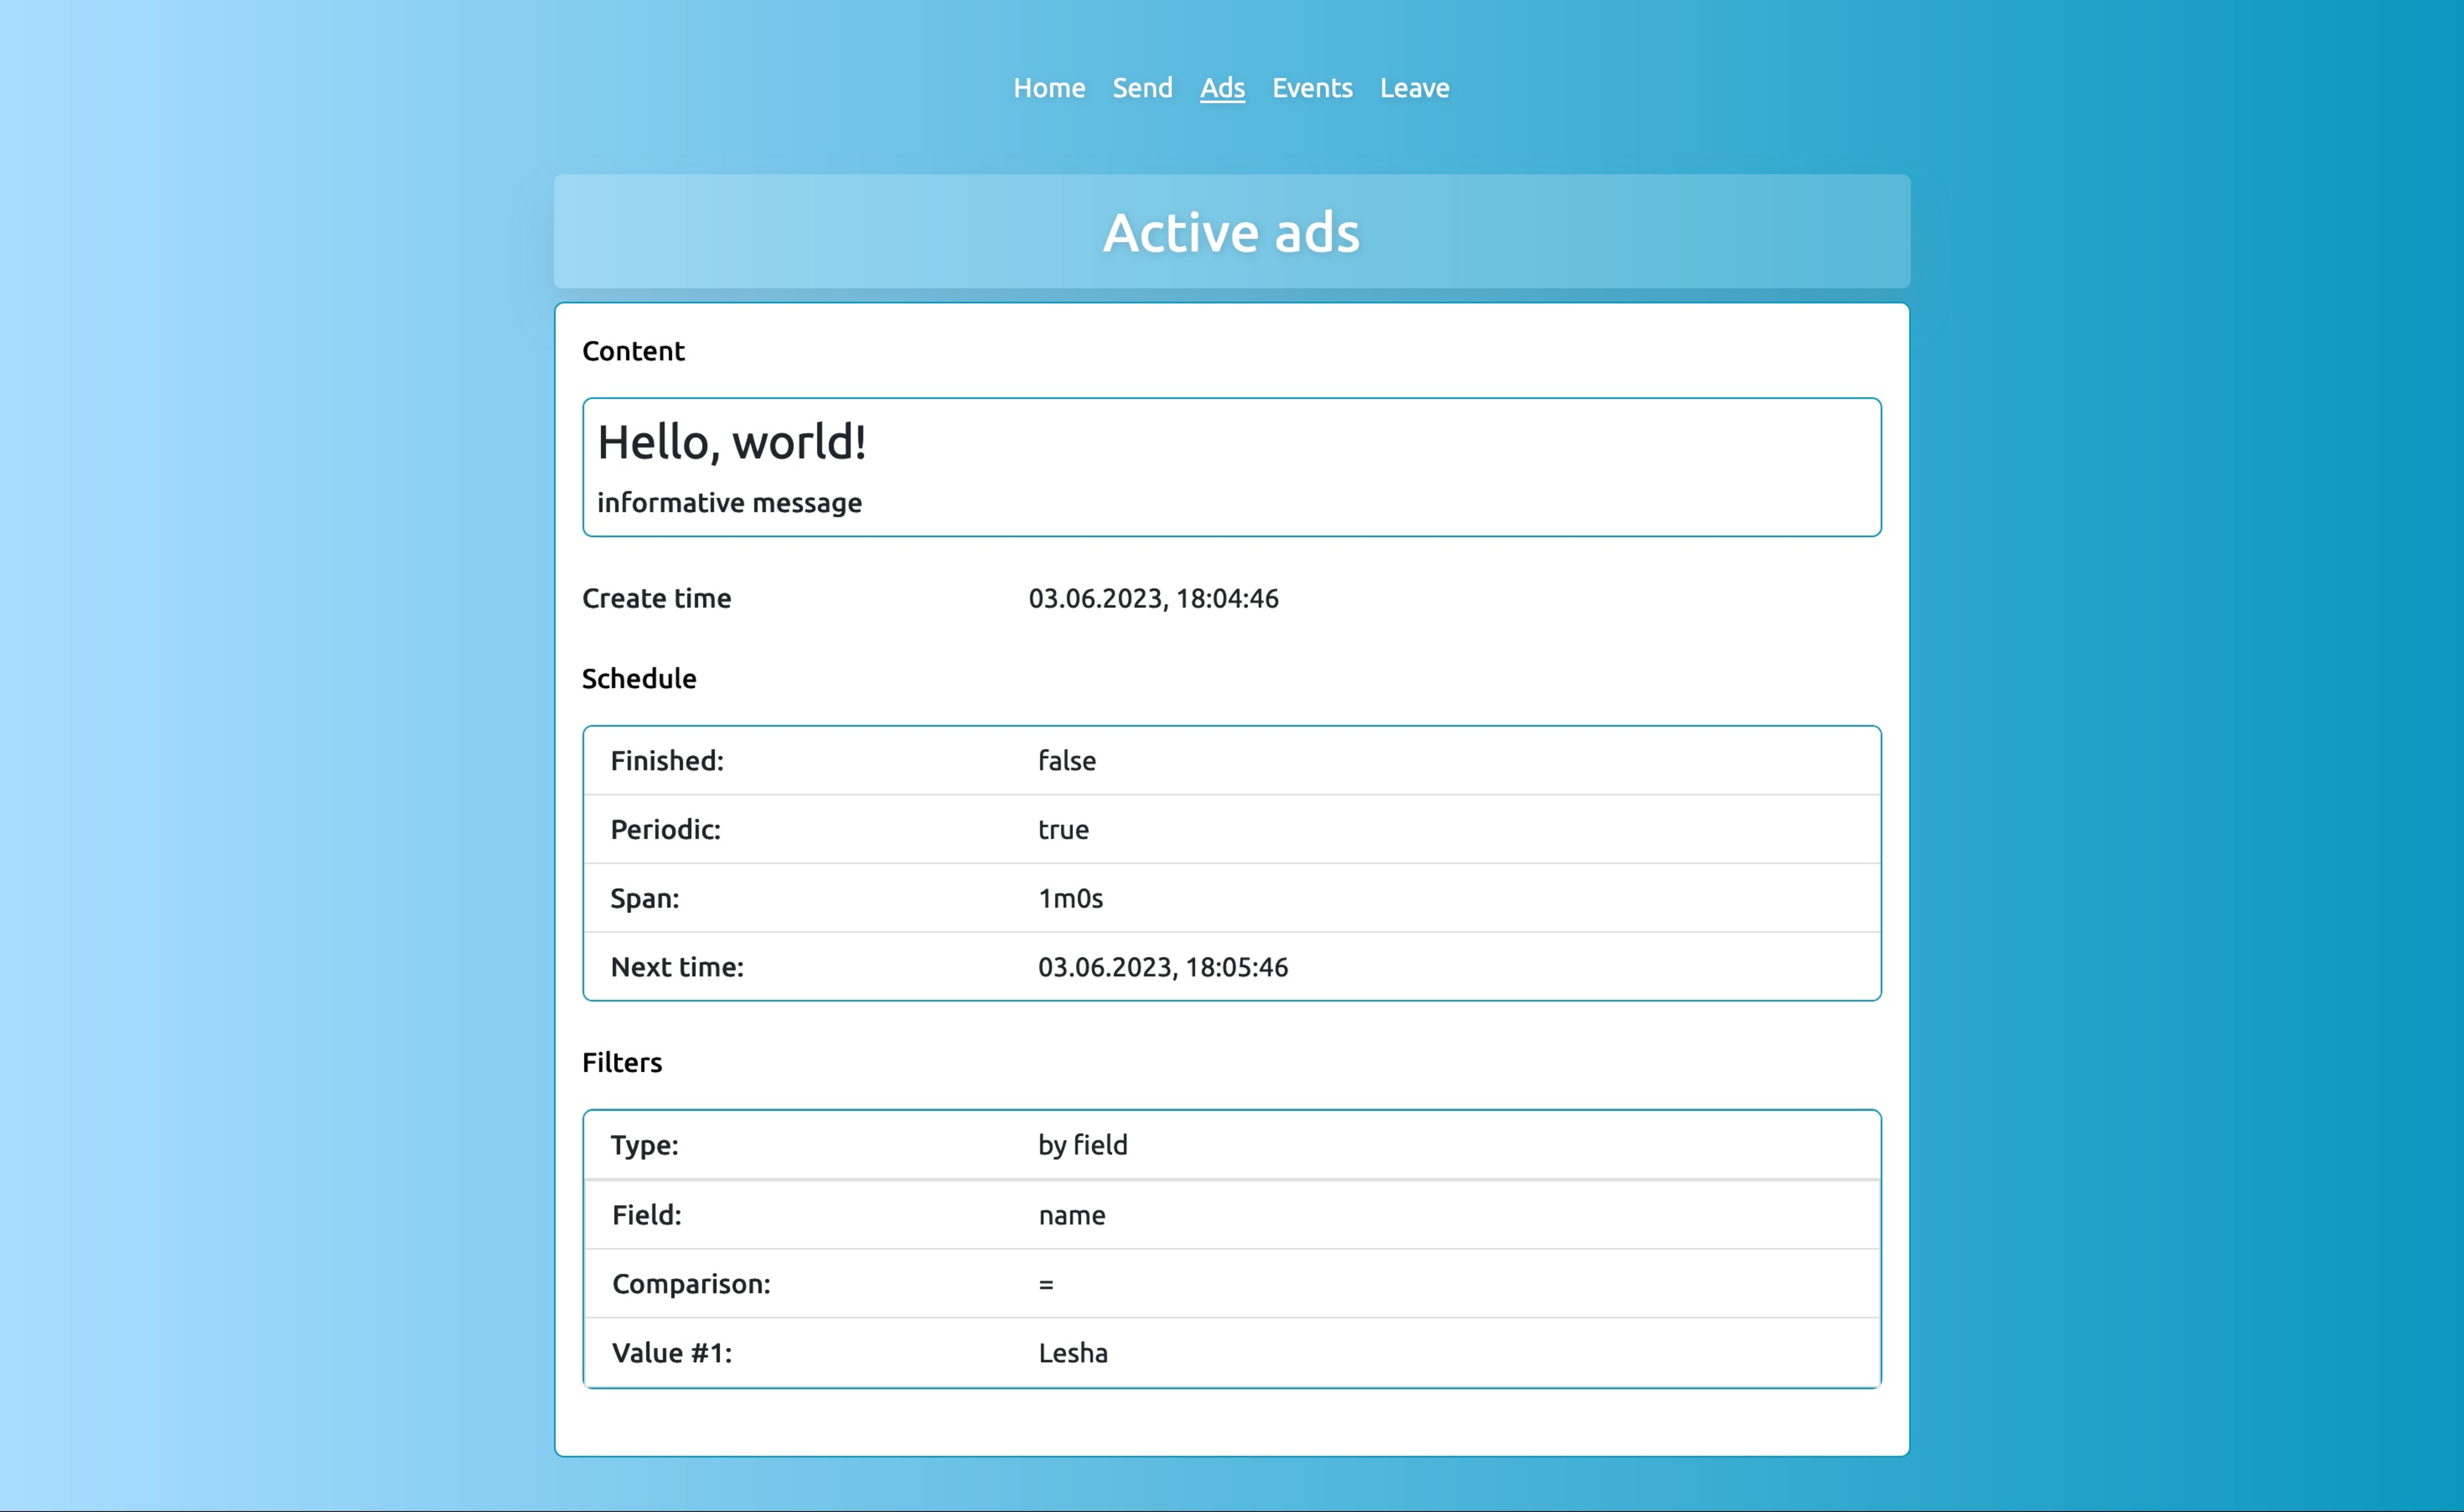
\includegraphics[width=0.8\linewidth]{./images/ads.pdf}
%%    \captionof{figure}{Страница просмотра списка незавершённых рассылок}
%%    \label{img:ads}
%%  \end{tabular}
%%\end{table}
%
%\newpage
%
%%\noindent
%
%\begin{figure}[h!]
%	\centering
%    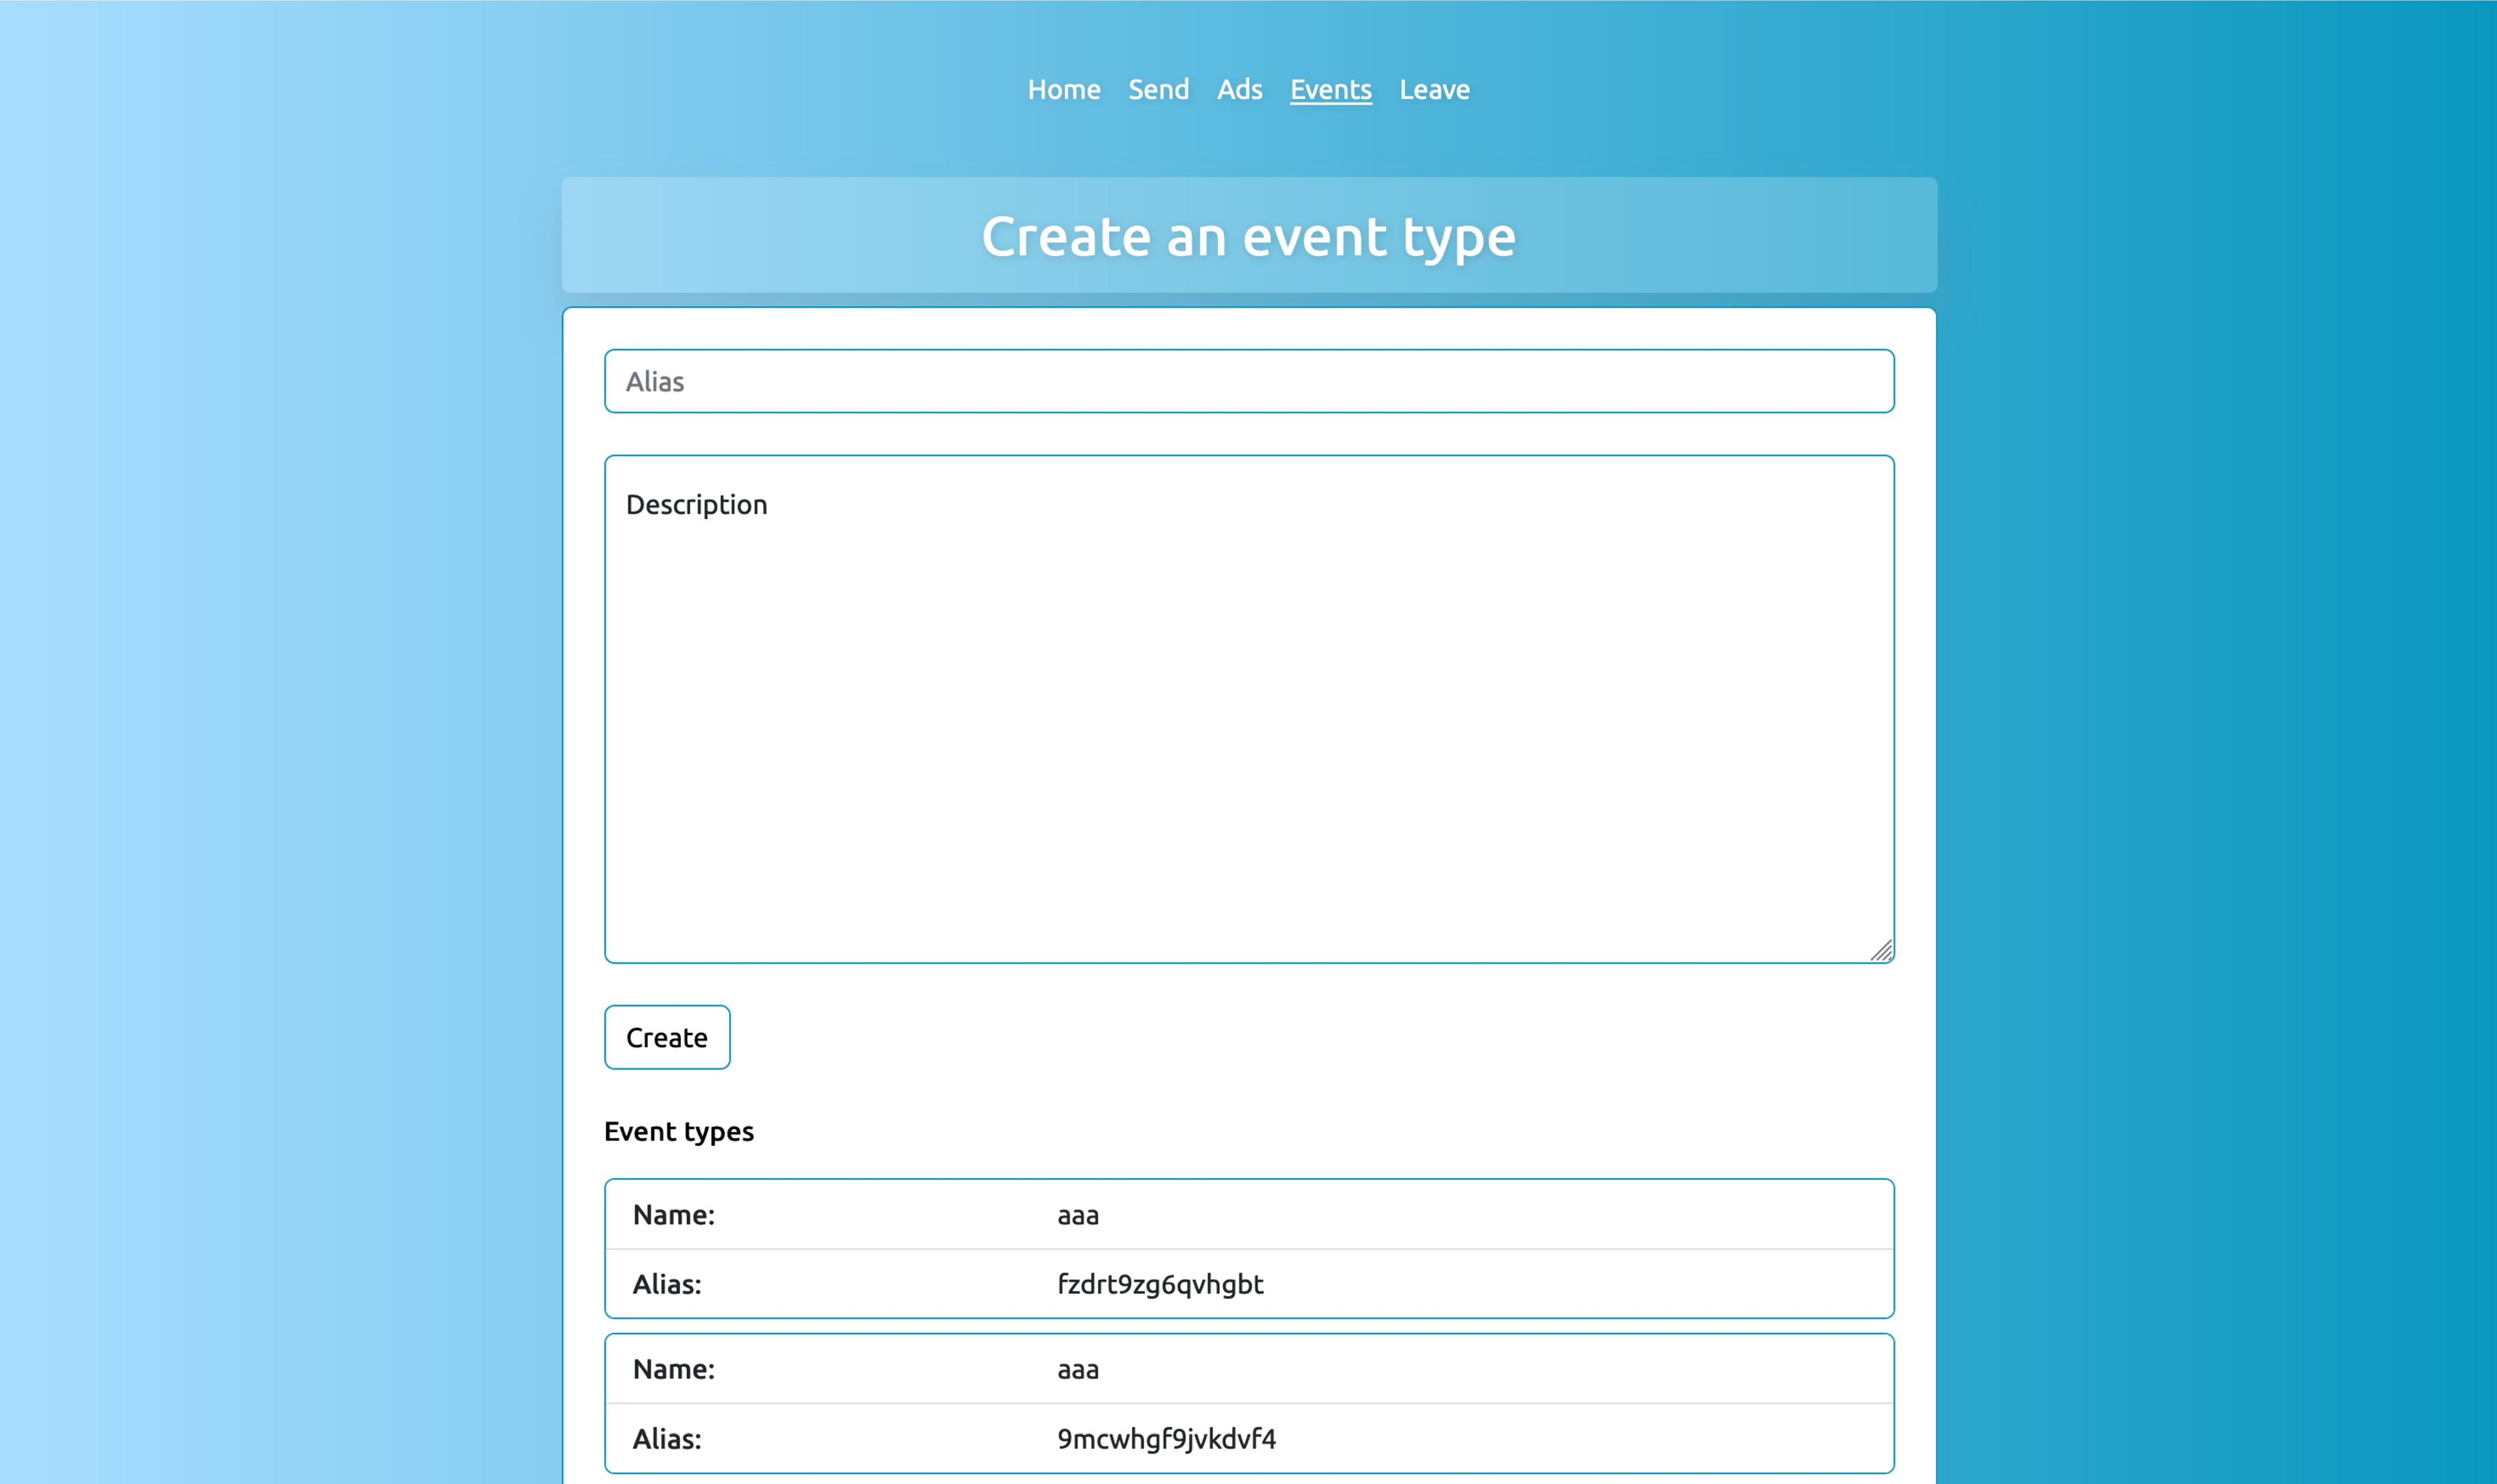
\includegraphics[width=0.9\linewidth]{./images/ets.pdf}
%    \caption{Страница просмотра и создания типов событий}
%    \label{img:ets}
%\end{figure}
%
%%\begin{table}[h!]
%%  \centering
%%  \begin{tabular}{p{1\linewidth}}
%%    \centering
%%    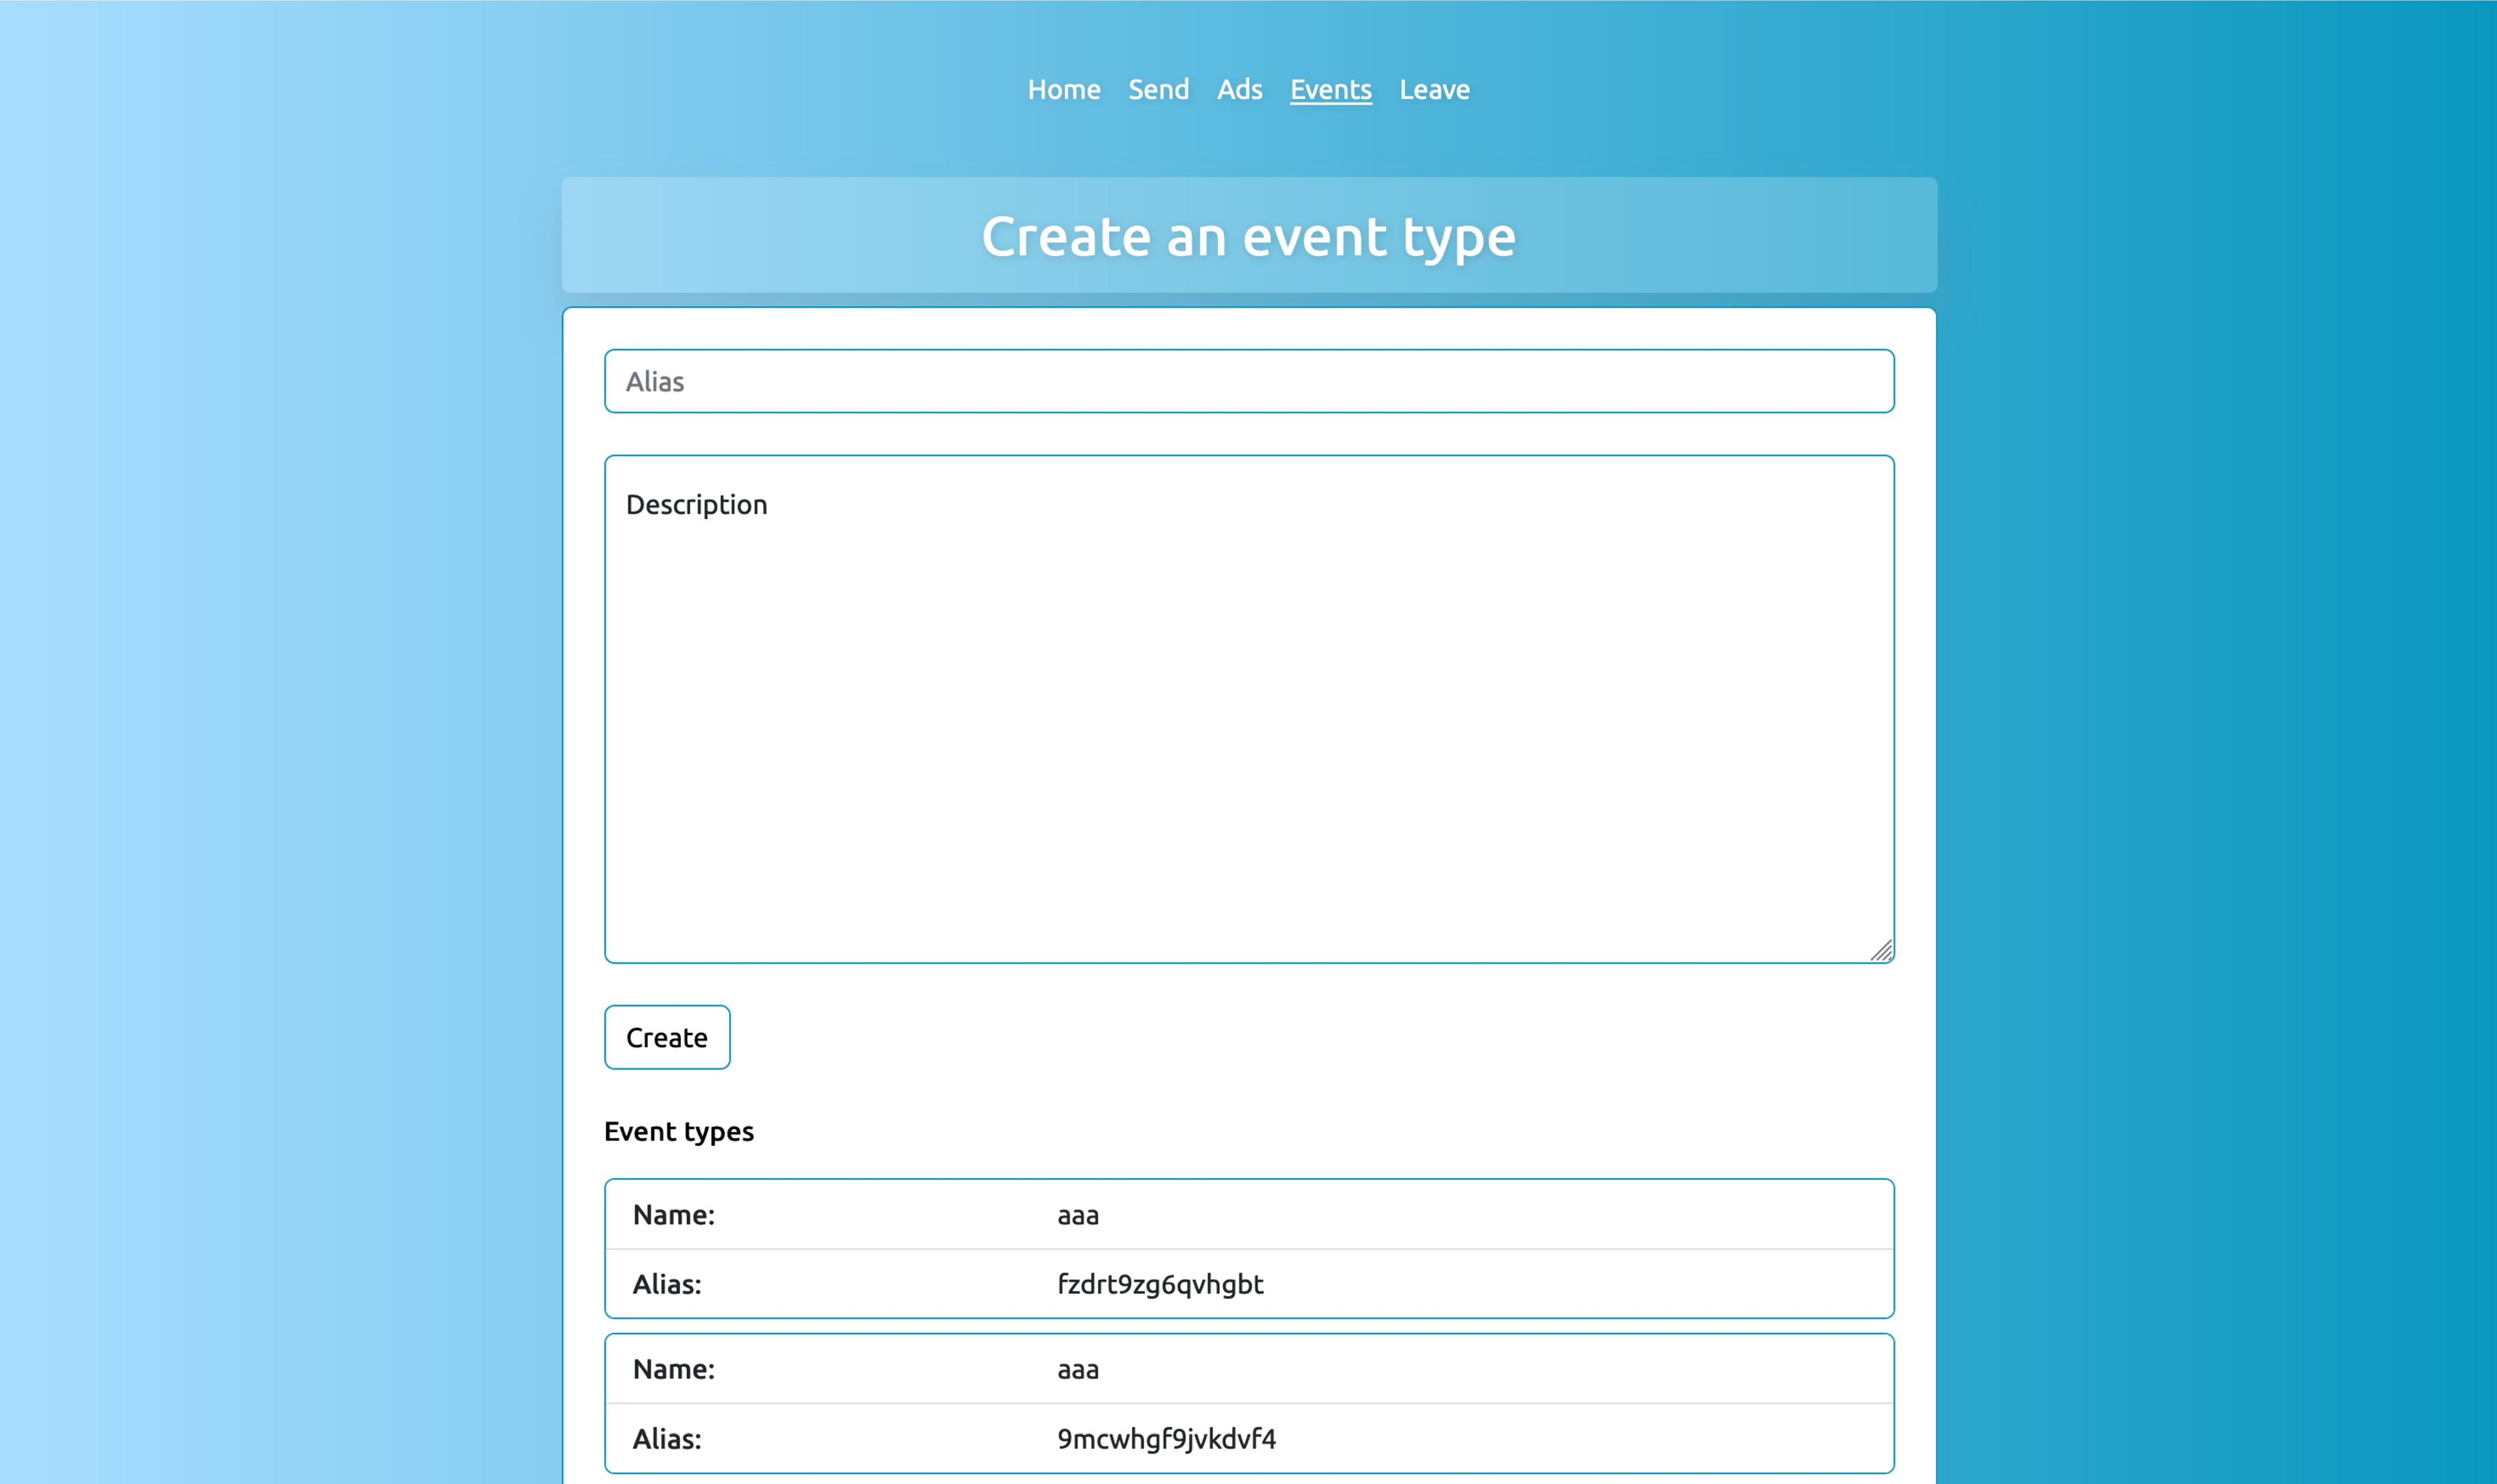
\includegraphics[width=0.9\linewidth]{./images/ets.pdf}
%%    \captionof{figure}{Страница просмотра и создания типов событий}
%%    \label{img:ets}
%%  \end{tabular}
%%\end{table}
%
%%\begin{table}[h!]
%%  \centering
%%  \begin{tabular}{p{1\linewidth}}
%%    \centering
%%    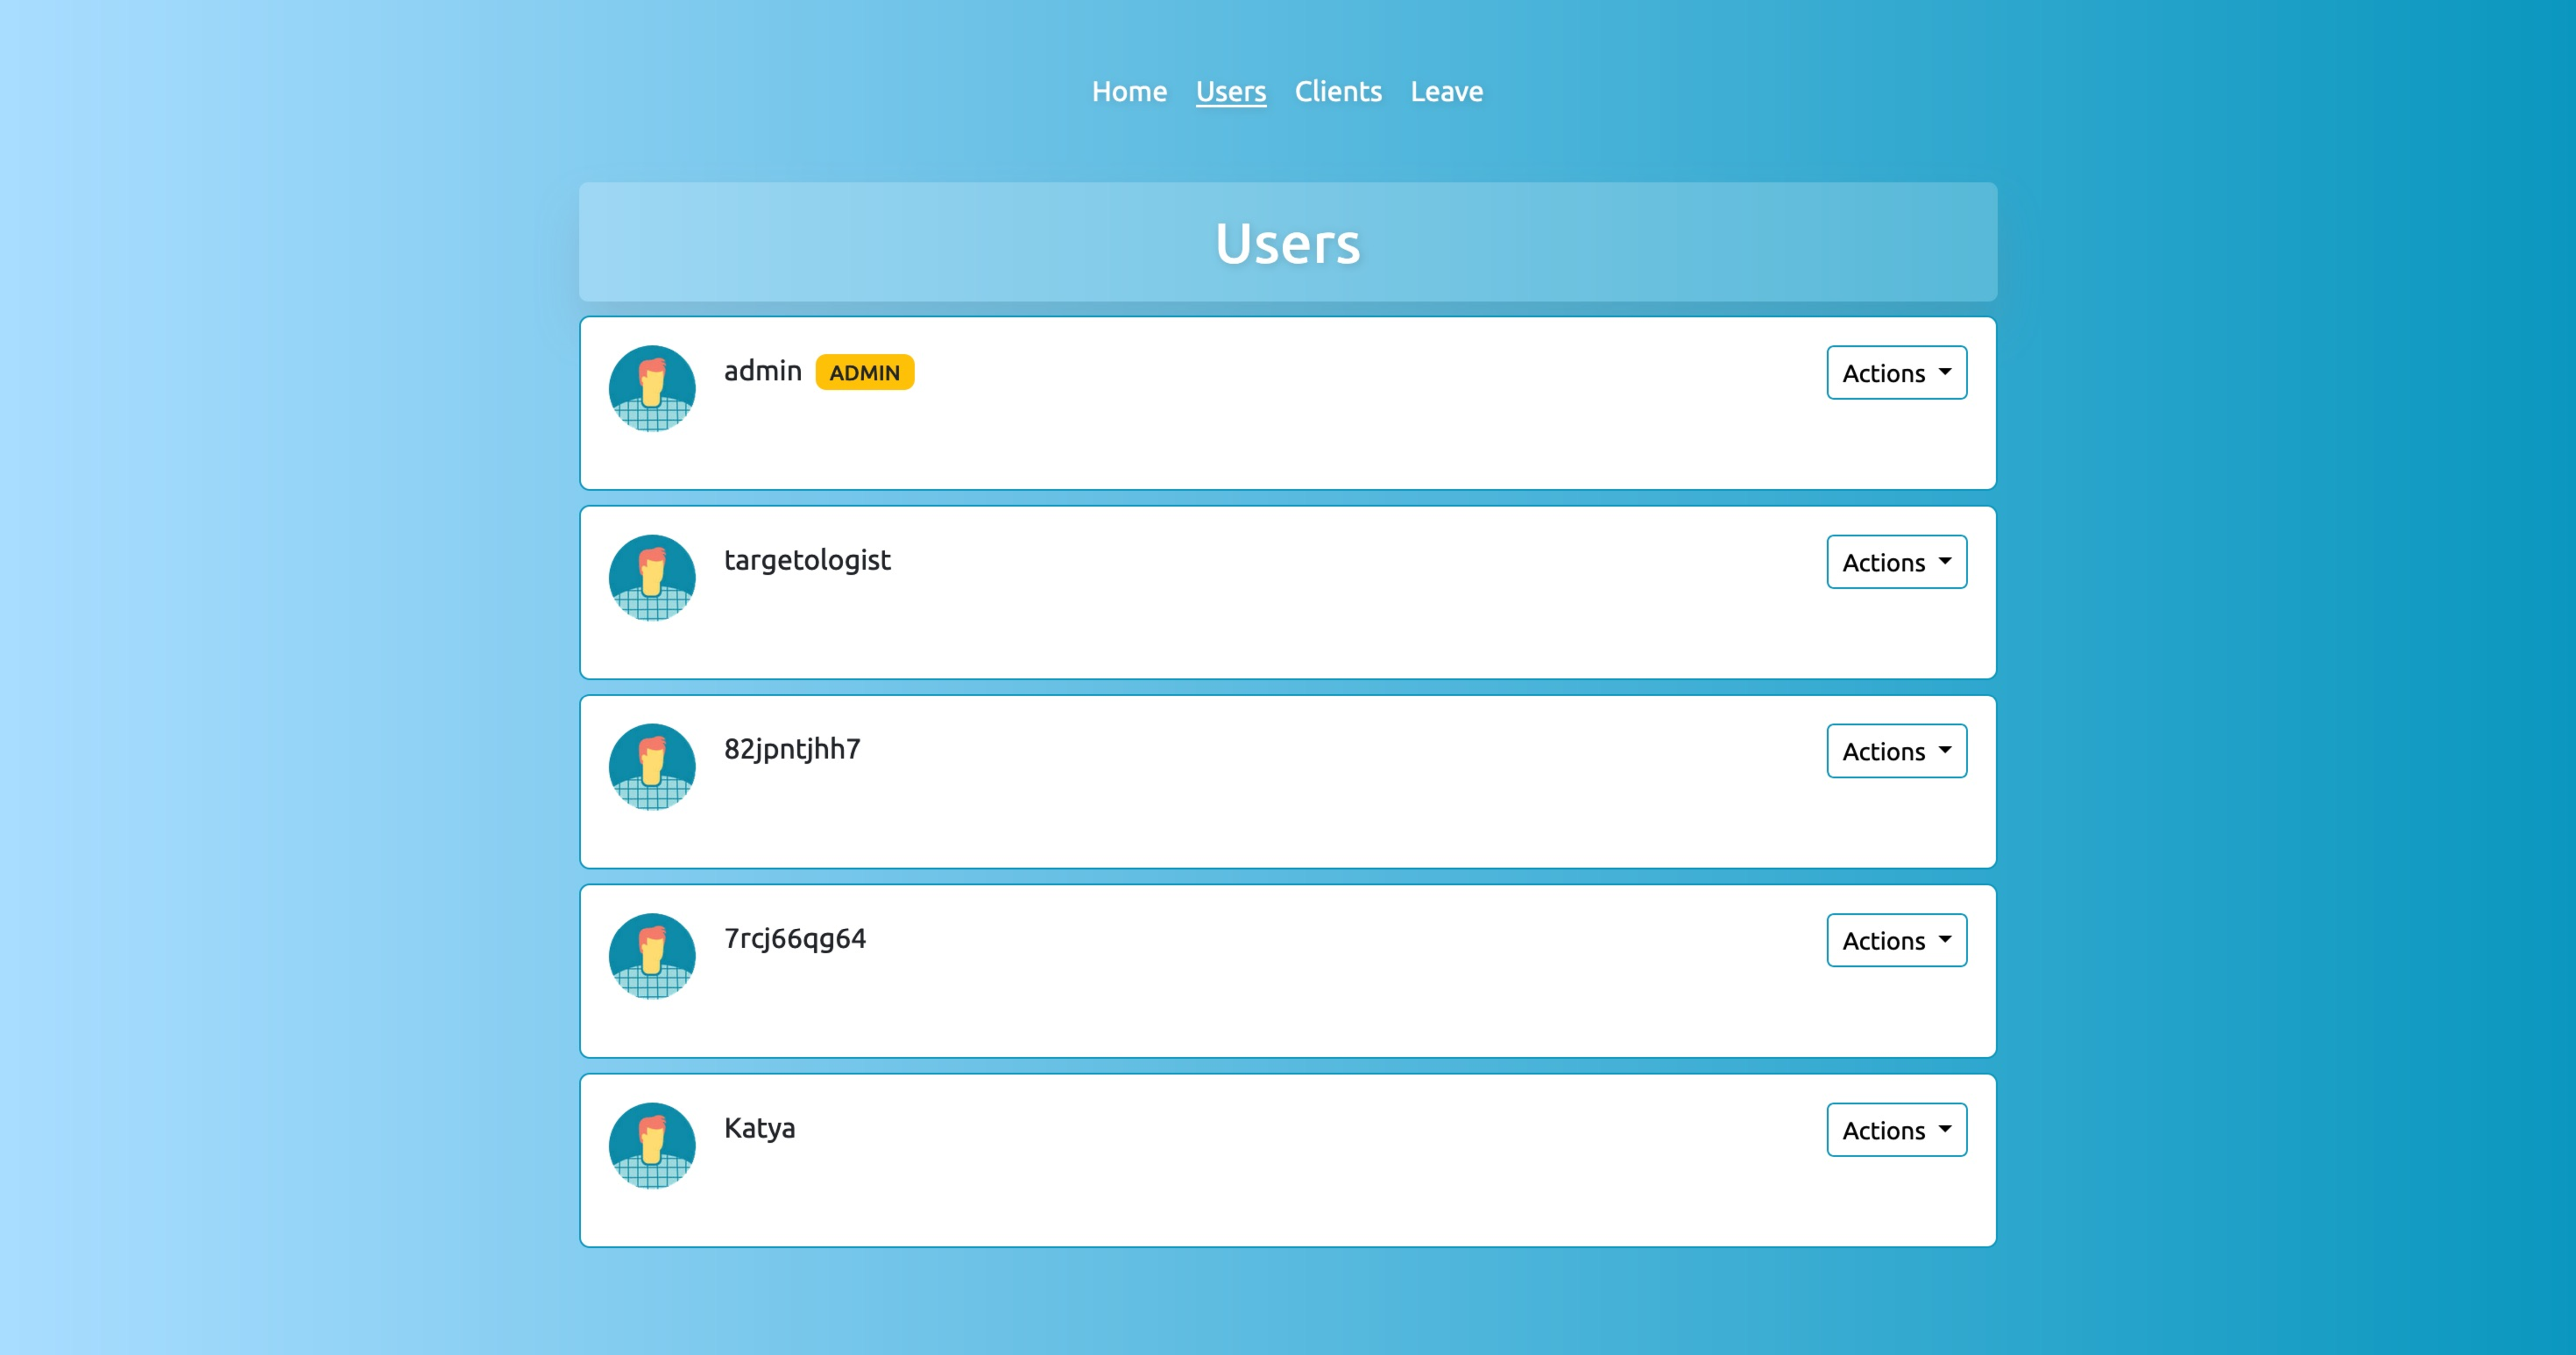
\includegraphics[width=0.6\linewidth]{./images/users.pdf}
%%    \captionof{figure}{Страница просмотра и редактирования списка пользователей}
%%    \label{img:users}
%%  \end{tabular}
%%\end{table}
%
%%\newpage
%
%\begin{table}[h!]
%  \centering
%  \begin{tabular}{p{1\linewidth}}
%    \centering
%    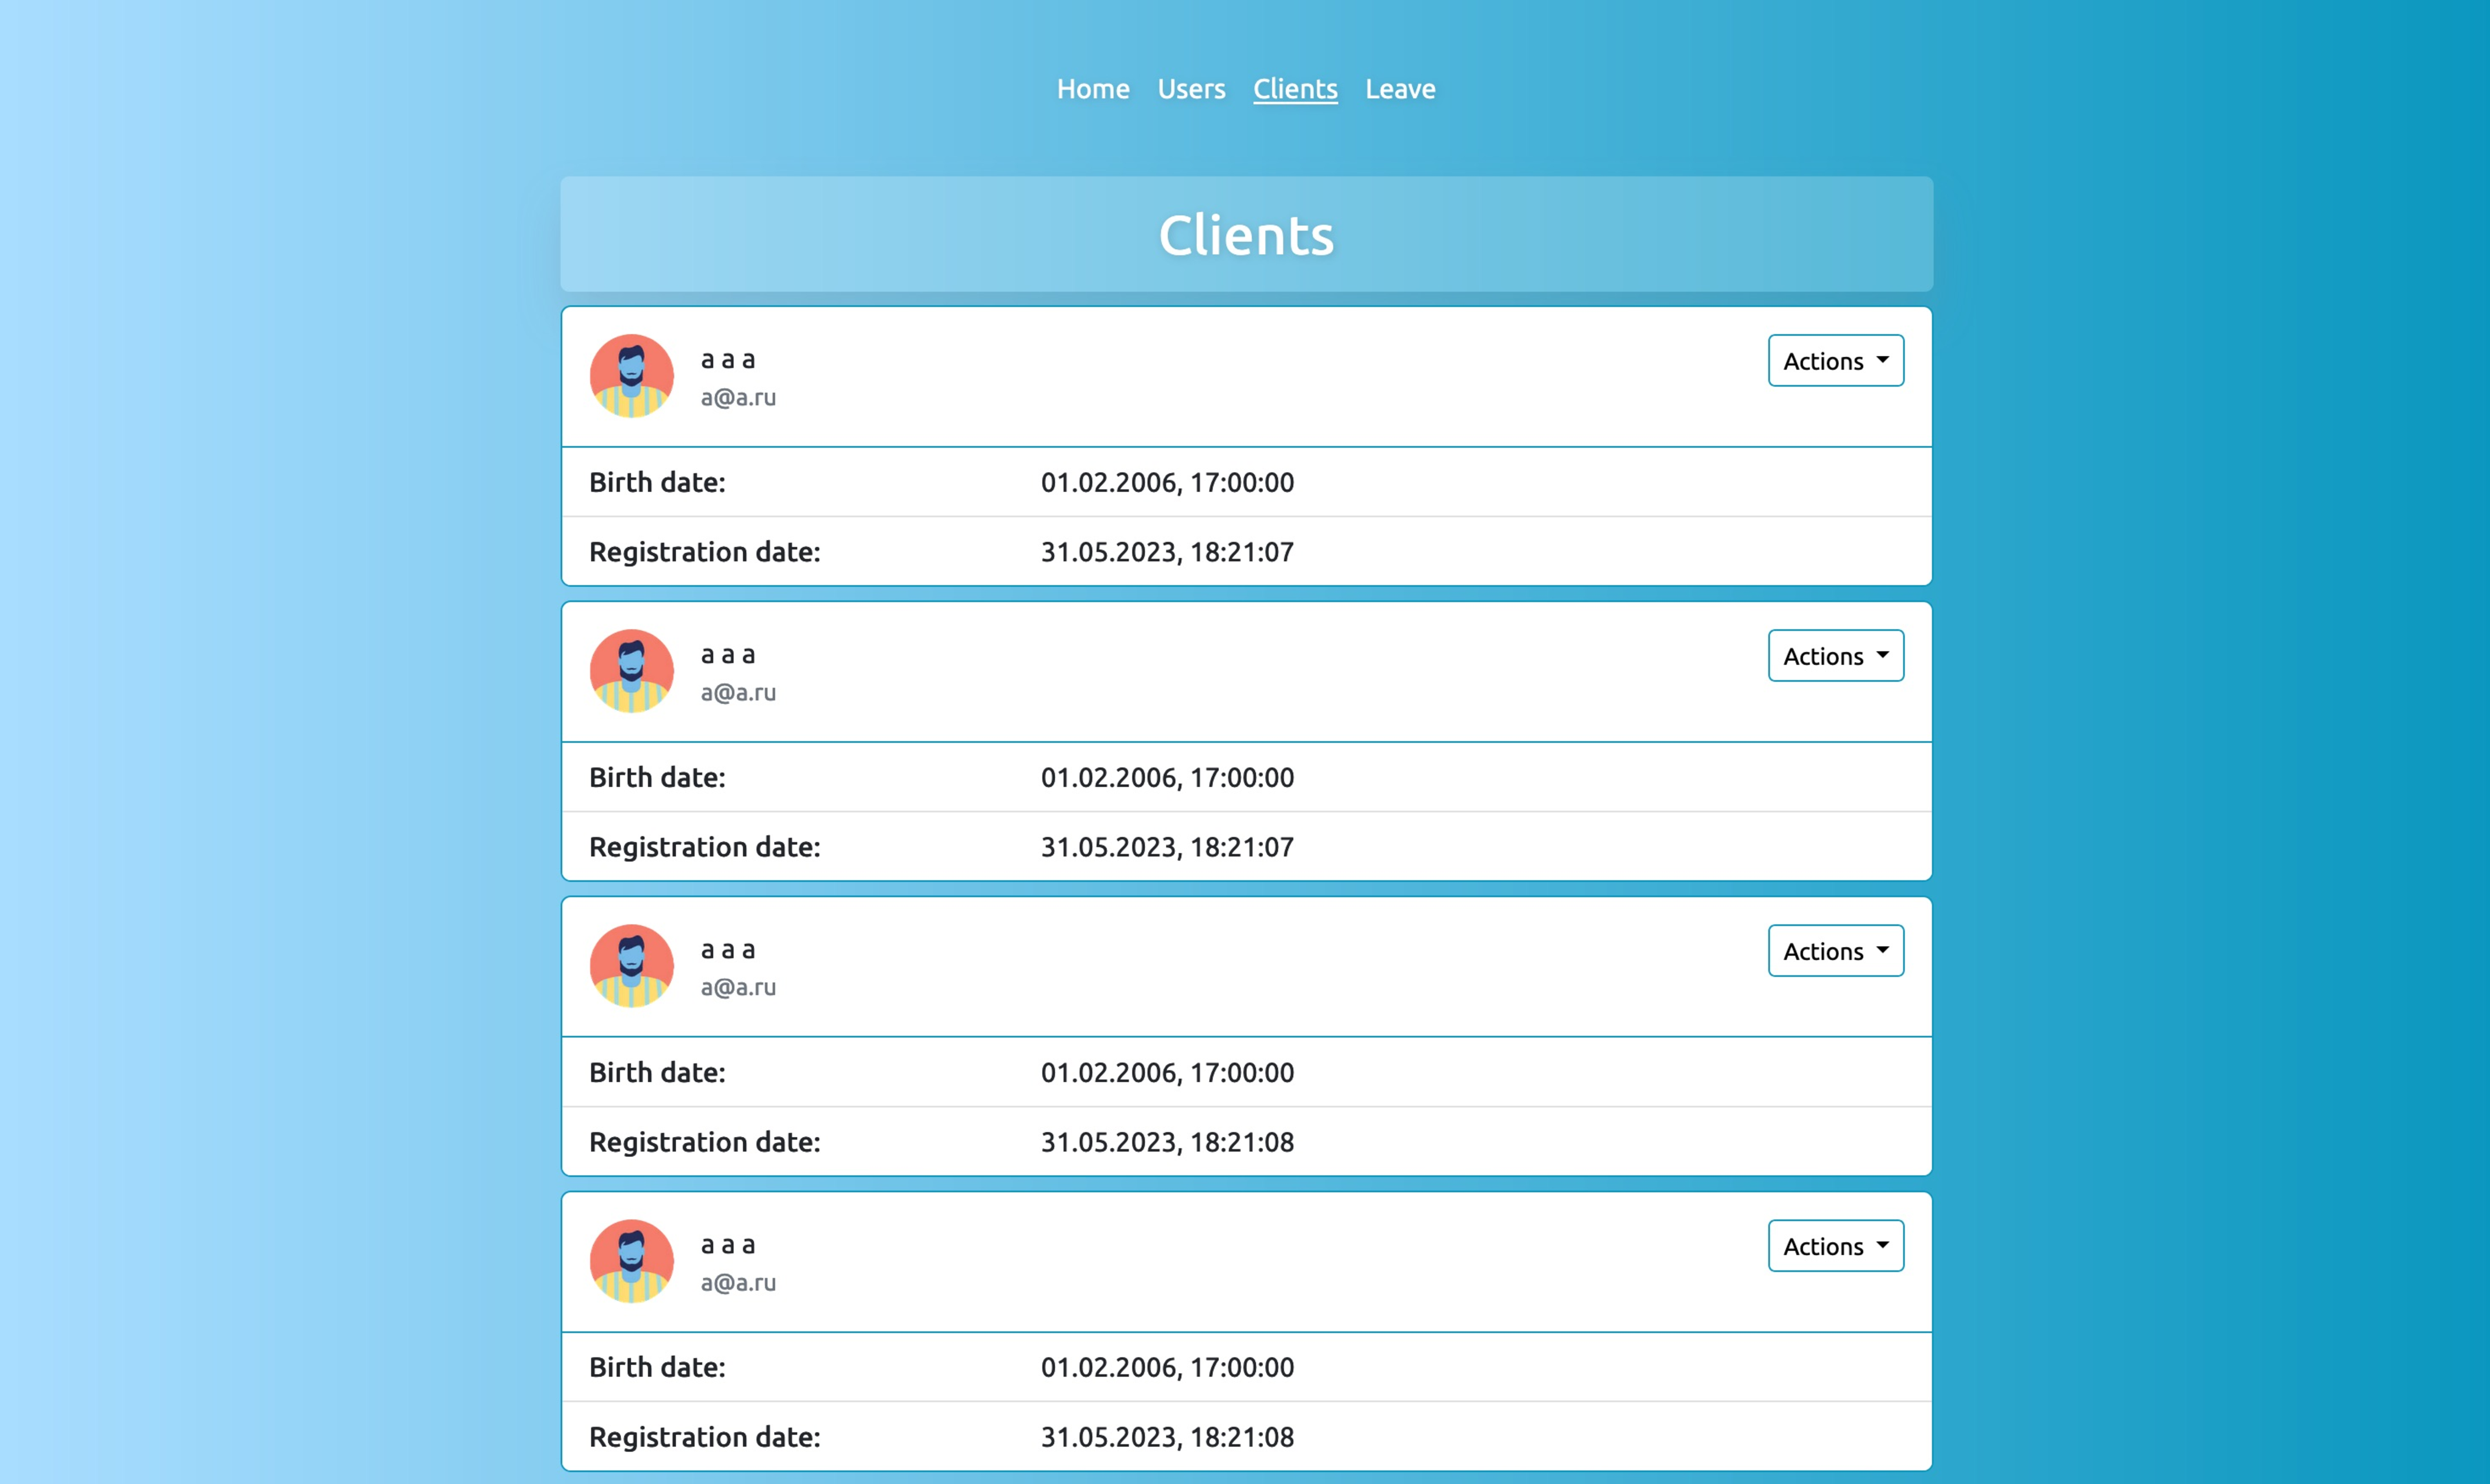
\includegraphics[width=0.9\linewidth]{./images/clients.pdf}
%    \captionof{figure}{Страница просмотра и редактирования списка клиентов}
%    \label{img:clients}
%  \end{tabular}
%\end{table}
%
%\newpage

\section{Тестирование}

Было проведено модульное тестирование функций модуля работы с пользователями системы при помощи стандартной библиотеки testing языка Golang. Модульные тесты обеспечивают полное покрытие функций авторизации, регистрации и входа в систему. В Приложении В приведена реализация одного из тестов для функции входа в систему.

Также, было проведено интеграционное тестирование функции получения информации о клиенте модуля работы с клиентами системы. Для каждой группы интеграционных тестов запускается Docker-контейнер с базой данных, которая при запуске заполняется тестовыми данными. SQL-скрипт для заполнения таблиц тестовыми данными, реализация функции запуска контейнера и реализация одного из тестов приведены в Приложении~В.

\section{Вывод}
В данном разделе был описан выбор систем управления базами данных. Были выбраны СУБД Postgres и ClickHouse, как наиболее полно удовлетворяющие поставленным задачам. Для аналитических данных будет использована СУБД ClickHouse, так как колоночные СУБД имеют большую производительность на запросах агрегации, для иных~---~Postgres. Также, описан выбор средств разработки серверной и клиентской частей ПО, для которых были выбраны Golang и Vue.js соответственно. Приведена таблица, описывающая интерфейс взаимодействия серверной и клиентской частей ПО и представлена общая схема взаимодействия компонентов системы. Описаны методы тестирования и обеспечения безопасности данных.







